%%% LaTeX Template
%%% This template can be used for both articles and reports.
%%%
%%% Copyright: http://www.howtotex.com/
%%% Date: February 2011

%%% Preamble
\documentclass[paper=a4, fontsize=11pt]{scrartcl}	% Article class of KOMA-script with 11pt font and a4 format

\usepackage[margin=0.7in]{geometry}
\setcounter{secnumdepth}{4}

\usepackage[english]{babel}															% English language/hyphenation
\usepackage[protrusion=true,expansion=true]{microtype}				% Better typography
\usepackage{amsmath,amsfonts,amsthm}										% Math packages
\usepackage[pdftex]{graphicx}														% Enable pdflatex
\usepackage{seqsplit}
%\usepackage{color,transparent}													% If you use color and/or transparency
\usepackage[hang, small,labelfont=bf,up,textfont=it,up]{caption}	% Custom captions under/above floats
\usepackage{epstopdf}																	% Converts .eps to .pdf
\usepackage{subfig}																		% Subfigures
\usepackage{booktabs}																	% Nicer tables


%%% Advanced verbatim environment
\usepackage{verbatim}
\usepackage{fancyvrb}
\DefineShortVerb{\|}								% delimiter to display inline verbatim text


%%% Custom sectioning (sectsty package)
\usepackage{sectsty}								% Custom sectioning (see below)
\allsectionsfont{%									% Change font of al section commands
	\usefont{OT1}{bch}{b}{n}%					% bch-b-n: CharterBT-Bold font
%	\hspace{15pt}%									% Uncomment for indentation
	}

\sectionfont{%										% Change font of \section command
	\usefont{OT1}{bch}{b}{n}%					% bch-b-n: CharterBT-Bold font
	\sectionrule{0pt}{0pt}{-5pt}{0.8pt}%	% Horizontal rule below section
	}


%%% Custom headers/footers (fancyhdr package)
\usepackage{fancyhdr}
\pagestyle{fancyplain}
\fancyhead{}														% No page header
\fancyfoot[C]{\thepage}										% Pagenumbering at center of footer
\renewcommand{\headrulewidth}{0pt}				% Remove header underlines
\renewcommand{\footrulewidth}{0pt}				% Remove footer underlines
\setlength{\headheight}{13.6pt}

%%% Equation and float numbering
\numberwithin{equation}{section}															% Equationnumbering: section.eq#
\numberwithin{figure}{section}																% Figurenumbering: section.fig#
\numberwithin{table}{section}																% Tablenumbering: section.tab#
\usepackage[parfill]{parskip}
\usepackage{float}
\usepackage{graphicx}
\usepackage{hyperref}
\usepackage[numbers]{natbib}

%%% Title
\title{ \vspace{-1in} 	\usefont{OT1}{bch}{b}{n}
		\huge \strut An Overview of the Recent Development of Indirect Inelastic Data Analysis in Mantid\strut \\
}
\author{ 									\usefont{OT1}{bch}{m}{n}
        Samuel Jackson\\		\usefont{OT1}{bch}{m}{n}
		ISIS Facility\\	\usefont{OT1}{bch}{m}{n}
        STFC Rutherford Appleton Laboratory\\
        \texttt{samuel.jackson@stfc.ac.uk}
}
\date{\today}

%%% Begin document
\begin{document}
\maketitle
\clearpage
\tableofcontents

\begin{abstract}
Mantid \cite{mantid}, the Manipulation and Analysis Toolkit for Instrument Data, is an open source and cross platform data analysis application specialising in Neutron and Muon scattering data. Recent development work has been undertaken to improve support for indirect geometry spectrometers, particularly in regards to those based at ISIS. This document aims to provide an overview of the current progress of development and describe from a technical perspective the procedures used in data reduction and analysis. The final section of the document then loosely outlines areas to focus on in further development in relation to the requirements described by instrument scientists.
\end{abstract}

\section{Introduction}
Mantid \cite{mantid} is an open source, cross platform framework for the analysis of Neutron and Muon scattering data. The project is primarily written in C++ with a Python API. The project includes a GUI based off of the QtiPlot project and primarily written using the Qt library.

Mantid aims to provide a single platform for neutron and muon scattering data analysis to all facilities across the world. It is developed by two teams of developers, one based at the ISIS facility at Rutherford Appleton Laboratory UK, the other at the Spallation Neutron Source (SNS) at Oak Ridge, Tennessee, USA. Recently additional partners from the Institut Laue-Langevin located in Grenoble and the Paul Scherrer Institute in Würenlingen, Switzerland have also contributed.

The project is currently still under heavy development and provides regular incremental releases for evaluation and feedback from instrument scientists and users in general and is therefore constantly evolving with each release. Until recently, Mantid operated on a three month release cycle. This has now been changed to so that the project releases every four months, with a longer emphasis on the testing and integration phase of development.

Time-of-flight neutron scattering instruments supported by Mantid, such as those based at ISIS and the SNS, can broadly be split into three categories based on the geometry of the instrument. In a direct instrument geometry the incident energy is fixed using choppers to select a specific incident wavelength directed towards the sample. Indirect or inverted geometry instruments use a polychromatic incident beam to scatter from the sample and select the final energy using a crystal analyser. Triple axis spectrometers use crystals both to moderate the incident beam and select the final energy of scattered neutrons \citep{fernandezalonso2013neutron}. This document focuses on the development progress of indirect geometry instruments within Mantid.

Up until now the indirect geometry section of Mantid has largely been based off of the the existing MODES application which in turn was based on OpenGenie \cite{wshowells2010} and the IRIS Data Analysis package \cite{wshowells1996}. The majority of the functionality has now been integrated into the Mantid framework in one form or another and we are now beginning to reach a point where we can expand the existing functionality further.

This document aims to give an overview of the current stage of development for the indirect geometry instruments section of the application as it currently exists in as much detail as possible to provide a historical snapshot of the progress so far. The remainder of the document then provides a weak outline of suggested directions for future development.

\section{Indirect Geometry Instruments}
Indirect geometry time-of-flight instruments, like the IRIS, OSIRIS, TOSCA, and VESUVIO spectrometers at ISIS are those in which the incident beam is polychromatic and crystal analysers are typically used to determine the final energy. Together these instruments cover a broad energy range. IRIS and OSIRIS operate in a low energy range of up to -0.4 to 0.4 meV (depending on the analyser used) and can be used to carry out Quasielastic neutron scattering around the elastic line. This is useful for studying the effects of diffusion  and tunneling. TOSCA covers the 0 to 500 meV range for investigating the lattice and intra-molecular structure of matter. VESUVIO operates at high energies of 5 - 150 eV and is used to perform deep inelastic neutron scattering. Diagram \ref{fig:instrument-energy-range} compares the energy range covered by the indirect geometry instruments at ISIS and the applicable techniques at each energy range.

\begin{figure}[H]
\centering
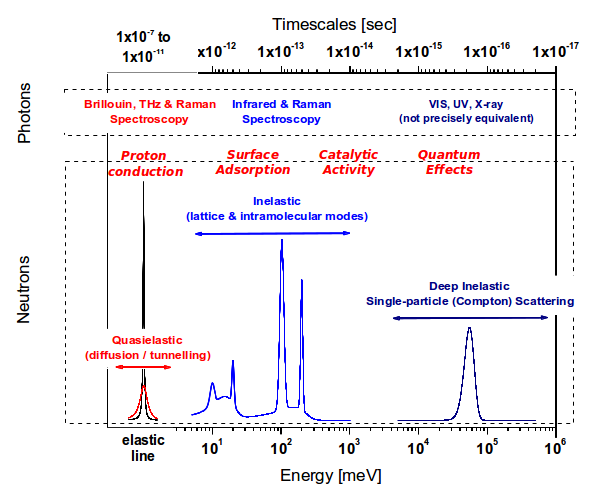
\includegraphics[width=0.6\textwidth]{img/instrument-energy-chart.png}
\caption{Energy ranges of various inelastic techniques. The ISIS instruments IRIS and OSIRIS cover the Quasielastic range, TOSCA covers the inelastic range and VESUVIO covers deep inelastic neutron scattering.}
\label{fig:instrument-energy-range}
\end{figure}

IRIS and OSIRIS share the N6 beamline in target station 1 at the ISIS facility. Both instruments are fed via curved guides from the source moderator. Two choppers positioned at 10m and 6.3m from the instruments define the incident wavelength band and prevent frame overlap \cite{smukhopadhyay2014}. TOSCA is located on the N4 beamline in ISIS target station 1 with a incident flight path of 17m and also has a chopper on the incoming beamline to prevent overlap and remove fast neutrons \cite{colognesi2002tosca}. VESUVIO is located on the S2 beamline and has an incident flight path of 11.005m \cite{mayers2011calibration}.

The final energy for inelastic instruments such as IRIS, OSIRIS and TOSCA is determined by the reflections from analyser crystals by means of Bragg scattering. IRIS and OSIRIS both have pyrolytic graphite crystal analysers with reflection planes 002 and 004 delivering a final energy of $E_f$=1.845 and 7.38 meV respectively \cite{adams2001iris, telling2003osiris}. This design leads to a resolution of 17.5 and 54.5 $\mu$eV for the 002 and 004 reflections on IRIS and 25 and 99 $\mu$eV on OSIRIS. IRIS additionally has a mica (muscovite or fluorinated) crystal analyser bank with reflections 002, 004, and 006, and $E_f$ corresponding to 0.207, 0.826, and 1.86 meV respectively which provide better resolutions (at the cost of intensity) of 11$\mu$eV (006), 4.5$\mu$eV (004) and
1.2$\mu$eV (002) compared to graphite. Recently, OSIRIS has had an upgrade which expands the operational energy range to -0.25 to 25 meV with the pyrolytic graphite analyser with reflection 002. The primary setting for both instruments is graphite with reflection 002. TOSCA has just a pyrolytic graphite analyser with 002 reflection \cite{colognesi2002tosca} and achieves a resolution of roughly 1.25\% of the measured energy transfer \cite{parker2003tosca}.

VESUVIO operates on the principle of neutron Compton scattering and uses a pair of gold foils which can be moved into different positions for use with the foil cycling technique described in \cite{schooneveld2006foil} which produces a neutron absorption resonance at 4.9 eV, emitting a $\gamma$-ray cascade which is detected by the instrument's Yttrium Aluminium Perovskite $\gamma$-ray detectors \cite{mayers2010user}.

\section{Theory}
Neutron scattering experiments are used to probe the structure of materials at a fundamental level. The results of such experiments can be used to learn a great deal about the internal structure of a sample and how it can behave under different conditions. In a neutron scattering experiment, a beam of neutrons is produced at a source (such as the one provided by ISIS) and directed to the various instruments attached to the beam line. These neutrons then scatter from the sample placed in the instrument. The angle and energy at which scattered neutrons are detected can then be used to deduce the structure and dynamics of the sample.

There are two main types of neutron scattering: elastic and inelastic. Elastic scattering is the special case when the final energy is equal to the incident energy and there is no energy transfer and the kinetic energy of the incident neutrons remain unchanged. Inelastic scattering is the more general case where some change in the kinetic energy of the incident neutron occurs and is useful for measuring the vibrations of atoms \cite{dssivia2011}.


\subsection{Data Reduction Theory}
Before data analysis can begin, the raw data collected from the instrument must be converted to an instrument independent function that describes the proportion of incident neutrons scattered with a given momentum and energy transfer known as $S(\mathbf{Q},\omega)$. Obviously, in order to calculate $S(\mathbf{Q},\omega)$ the quantities of \textbf{Q} (wavevector transfer) and $\omega$ (energy transfer) must first be derived.

\mbox{ }\\
\begin{figure}[H]
\centering
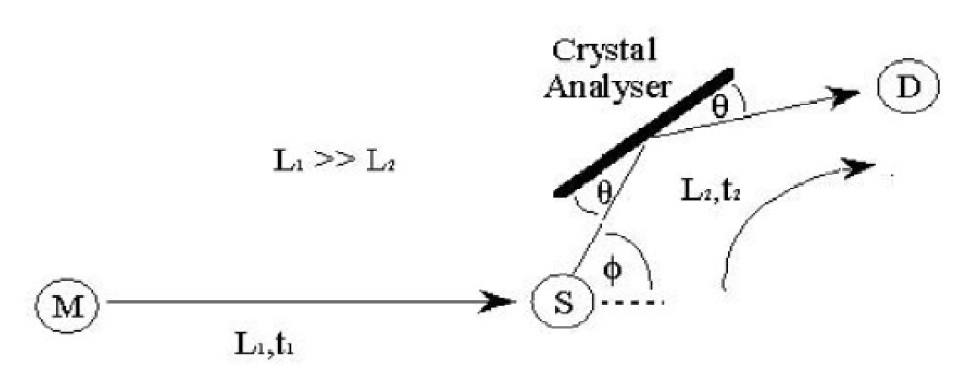
\includegraphics[width=0.7\textwidth]{img/instrument-diagram.png}
\caption{Diagram of the basic principle of an inelastic neutron scattering experiment. M is the moderator, S is the sample, and D is the detector \cite{smukhopadhyay2014}}
\label{fig:instrument-setup}
\end{figure}

In order to convert the raw data collected from the instrument from time-of-flight measurements to energy transfer the routine uses known parameters about the instrument as illustrated in figure \ref{fig:instrument-setup}. The raw time-of-flight data is recorded in counts per microsecond and can be calculated using the parameters of the instrument with the time-of-flight equation:

\begin{equation}
\label{eq:time-of-flight}
t = \frac{L_1}{V_1} + \frac{L_2}{V_2}
\end{equation}

Where $L_1$ is the distance between moderator and sample, $L_2$ is the distance between the sample and detector, $V_1$ and $V_2$ are the incident and final velocities of a neutron. The final energy detected by a detector can be written in terms of a neutron's mass ($m_{n}$) and velocity ($v$) from the sample to the detector:

\begin{equation}
E_f = \frac{1}{2}m_{n}v^2 = \frac{1}{2}m_{n} ( L_2 / t_2 ) ^2
\end{equation}

Which can also be written in terms of the distance between sample and detector ($L_2$) and the corresponding time-of-flight over this distance ($t_2$). To calculate the transfer of energy knowledge of the flight path between the moderator and sample ($L_1$) and the time of flight over this distance ($t_1$) can be used to calculate the incident energy using equation above. In indirect geometry instruments, the final energy is fixed by the crystal analysers which filters any neutrons with wavelengths not satisfying the Bragg condition:

\begin{equation}
\label{eq:braggs-law}
\lambda = 2dsin(\theta)
\end{equation}

Where $\lambda$ is the neutrons wavelength, $d$ is the spacing between planes in the crystal lattice, and $\theta$ is the scattering angle. The transfer of energy is then simple the difference between incident and final energy:

\begin{equation}
\Delta E = E_i - E_f = \frac{1}{2}m_n[(L_1 / t_1-t_2)^2 - (L_1/t_2)^2]
\end{equation}

This is the basic theory behind the convert to energy reduction routine described in section \ref{sec:energy-transfer}. Momentum transfer \textbf{Q}, is defined as the difference between the final and incident wave vectors.

\begin{equation}
\mathbf{Q} = k_f - k_i
\end{equation}

Where $k_i$ and $k_f$ are the incident and final wave vectors. The magnitude of \textbf{Q} is defined as:

\begin{equation}
Q^2 = k_i^2 + k_f^2 - 2k_ik_fcos 2\theta
\end{equation}

Where $\theta$ is the scattering angle of the sample \citep{dssivia2011}. In reality, the $S(\mathbf{Q}, \omega)$ cannot be directly measured by experiment because of the resolution of the instrument. Instead, the quantity measured from the instrument (denoted $I(\mathbf{Q}, \omega)$) is a convolution between the scattering function and the instrument resolution:

\begin{equation}
\label{eq:instrument-result}
I(\mathbf{Q}, \omega) = S(\mathbf{Q}, \omega) \otimes R(\mathbf{Q}, \omega)
\end{equation}

Where $S(\mathbf{Q}, \omega)$ is given by:

\begin{equation}
S(\mathbf{Q}, \omega) = \Sigma_j \frac{b_j}{M_j}^2Q^2 < u_j >^2 e^{-2W}\frac{Z(\omega)}{\hbar\omega}
\end{equation}

Where $b_j$ is the neutron scattering length of the atom, $M_j$ is the mass of the atom, $< u_j >$ is the amplitude of vibration of each atom,  $Z(\omega)$ density of states of a molecule, and $e^{-2W}$ is the Debye-Waller factor \cite{smukhopadhyay2014} to correct for thermal energy in which $W$ is equal to:

\begin{equation}
W = \frac{1}{2} < u^2_{MSD} > Q^2
\end{equation}

And $< u^2_{MSD} >$ is the mean squared displacement of the scattering atom. The mean squared displacement is the quantity that is analysed using the MSDFit routine described in section \ref{subsubsec:msdfit}.

This theory is only relevant for IRIS, OSIRIS, and TOSCA spectrometers. The theory behind data reduction for the deep inelastic neutron scattering instrument VESUVIO is completely different and is based on the validity of the impulse approximation at sufficiently high energy and momentum transfer. A detailed description of the theory behind data analysis and reduction for VEUSVIO can be found in Ref. \cite{mayers2012vesuvio}.

\subsubsection{Diffraction Reduction}
In the case of diffraction experiments, there is no need to convert to energy transfer or $S(\mathbf{Q}, \omega)$. Instead, the results are converted from the raw time-of-flight data to $d$-spacing, the distance between the planes in a lattice. Results are calculated using known parameters of the instrument via the time-of-flight equation (equation \ref{eq:time-of-flight}) and Bragg's law (equation \ref{eq:braggs-law}). Diffraction experiments may be run either on their own or in parallel with spectroscopy.

At pulsed time-of-flight sources such as ISIS a wavelength scanning method can be used to determine the scattering vector by varying the wavelength of the incident wavevector and keeping the scattering angle constant thereby satisfying the Bragg condition \citep{fernandezalonso2013neutron}:

\begin{equation}
\label{eq:bragg-condition}
\textbf{Q} = 4\pi sin(\theta)/\lambda
\end{equation}

Using equations \ref{eq:braggs-law} and \ref{eq:time-of-flight}, the $d$-spacing of a sample is given as a function of the scattering angle $\theta$ and distances between the source and sample $L_0$ and sample and detector $L_1$:

\begin{equation}
d = \frac{2 t sin(\theta)M_n (L_0 + L_1)}{h}
\end{equation}

Where $t$ is the time of flight, $M_n$ is the mass of a neutron and $h$ is the Planck constant.
 
\subsection{Data Analysis Theory}

\subsubsection{Convolution Theory}
Data analysis of inelastic scattering data is primarily concerned with separating the scattering function for the instrument's resolution function in the relation defined in equation \ref{eq:instrument-result} . In theory, these can then be separated through the deconvolution of the two functions. There are several different functional forms that may occur depending on the sample used:

\begin{itemize}
\item The simplest case is when there is a simple diffusive motion within the sample $S(\mathbf{Q},\omega)$ and $R(\mathbf{Q},\omega)$ will both have the form of a Lorentzian and hence there convolution will also be a Lorentzian.

\item The second case is when both the scattering function and the resolution function both have simple functional forms. For example, when $S(\mathbf{Q},\omega)$ is a Lorenztian and $R(\mathbf{Q},\omega)$ is a Gaussian.

\item The final case is when $R(\mathbf{Q}, \omega)$ does not have a simple functional form, and so must be convoluted numerically with the $S(\mathbf{Q}, \omega)$.
\end{itemize}

The typical way to handle the latter case is through fitting the appropriate model to the convoluted data and is the purpose of the ConvFit interface described in section \ref{subsubsec:convfit} which provides a least-squares fit to the convolution of the measured data and the resolution.

An alternative method of deconvolution of the scattering and resolution functions is through the intermediate scattering function, denoted $I(\mathbf{Q}, t)$ which is proportional to the Fourier transform of the scattering and resolution functions:

\begin{equation}
I(\mathbf{Q}, t) = S(\mathbf{Q}, t) \times R(\mathbf{Q}, t)
\end{equation}

As the resolution of the instrument is known, the intermediate scattering function can be divided by the resolution and back transformed to obtain the scattering function. This method has the advantage in that the form of the function does not have to be assumed as in ConvFit, but the back transformation from $S(\mathbf{Q}, t)$ to the true scattering function is problematic due to the phase problem \citep{dssivia2011} and the propagation of statistical errors \citep{wild1977measurement}. The Fury routine provides an interface to perform a Fourier transform on the measured data and resolution, but does not provide an automated back transformation because of the aforementioned issues.

\subsubsection{Bayesian Analysis}
An alternative method to model fitting is the use of Bayesian methods to select the best model for the data based on a choice of possible functions. One method described by Sivia \citep{dssivia1992} selects the most likely choice of model from sum of a $\delta$-function and zero or more Lorentzians convolved with the resolution function of the instrument. Using this method, the number of Lorentzians is iteratively varied and the optimum number selected as the final model. An extension of this method replaces the sum of Lorentzians with a single stretched exponential function. For each group of spectra, the best value for the $\beta$ and $\Gamma$ parameters is obtained \citep{wshowells2010}. This model can be used to fit the shape resulting from polymer samples \citep{wshowells1996, higgins1977observation, higgins1977q}, and is the basis behind the Stretch program described in section \ref{subsec:stretch}.

From the width parameters of the selected model diffusion can be interpreted. This is typically done by modelling jump diffusion where it is assumed an atom remains at a given site for a length of time before moving rapidly to a new site in a time that is negligible to the time spent being stationary. There are several different models for diffusion depending on the application. The Chudley-Elliott form assumes the atom jumps from one point to its nearest neighbour site $l$ distance away in a Bravis lattice \citep{chudley1961neutron} and has the form:

\begin{equation}
\Gamma(Q) = (\hbar/\pi t) \cdot (1 - sin(Ql)/Ql)/\tau
\end{equation}

The Hall-Ross \citep{hall1981incoherent} form models the diffusive jump motion as several steps and do oscillatory motion at alternate sites.

\begin{equation}
\Gamma(Q) = (\hbar/\pi t) \cdot (1-exp(-lQ^2))/\tau
\end{equation}

Teixeria's model \citep{teixeira1985experimental} is used to study the dynamics of super cooled water and has the form:

\begin{equation}
\Gamma(Q) = DQ^2/(1 + DQ^2\tau)
\end{equation}

Where the diffusion constant $D$ is equal to:

\begin{equation}
D=<l^2>/6\tau
\end{equation}

Finally the Fick diffusion model \citep{fick1855v} has the form:

\begin{equation}
\Gamma(Q) = DQ^2
\end{equation}

Each of these functions are implemented as part of the JumpFit interface (section \ref{subsec:jumpfit}), but are also available through the generic fit wizard in Mantid.

\subsubsection{Absorption Corrections}
A sample typically must be corrected for absorption by the sample and by its container. Typically a sample will need to be corrected for flat plate geometry \citep{ccarlile1974} or cylindrical geometry \citep{aksoper1989}. The methods for cylindrical geometry used in Mantid have been adapted from the methods described in the ATLAS manual \citep{aksoper1989}.

Absorption corrections use the formalism specified by Paalman and Pings \citep{hhpaalman1962} to describe the attenuation factors of a sample/container. They are denoted by $A_{i,j}$ where $i$ refers to scattering and $j$ refers to attenuation. For example, $A_{s,sc}$ is the attenuation factor for scattering in the sample plus container. The scattering cross sections for the sample and container are denoted as $\Sigma_s$ and $\Sigma_c$. The scattering from an empty container is then given by:

\begin{equation}
I_c = \Sigma_c A_{c,c}
\end{equation}

Scattering from the sample plus the container is then given by:

\begin{equation}
I_{sc} = \Sigma_s A_{s,sc} + \Sigma_c A_{c,sc}
\end{equation}

The scattering cross section for the sample can the be calculated as:

\begin{equation}
\Sigma_s = (I_{sc}I_cA_{c,sc}/A_{c,c}) / A_{s,sc}
\end{equation}

There are two routines in Mantid which perform these corrections. Calculate Corrections calculates the attenuation parameters $A_{i,j}$, while Apply Corrections uses them to calculate $\Sigma_s$ based on the geometry as described here.

\section{Data Reduction with Mantid}
Mantid provides a collection of graphical user interfaces to specialised indirect inelastic data reduction routines under the menu \textit{Interfaces \textgreater Indirect}. The majority of these routines are based on or directly ported from the MODES3 and IRIS Data Analysis (IDA) packages \citep{wshowells2010, wshowells1996}. As such, the core of the functionality of these routines has mostly remained the same, but the implementation has changed. This section outlines the current development of each of the interfaces and routines available.

The Convert to Energy interface provides the initial entry point for data into Mantid for indirect instruments. The functionality of this interface is currently also shared with the direct instruments, although a separation of the interfaces is planned in future releases.

The code for data  reduction programs are primarily stored in the inelastic scripts folder of the Mantid installation (\textit{\textless Installation Directory\textgreater /Mantid/scripts/Inelastic}). The energy conversion reducer is in a file called inelastic\_indirect\_reducer.py while the diffraction reducer is in IndirectDiffractionReduction.py. The reduction steps used by both are in inelastic\_indirect\_reduction\_steps.py. The generic reducer class is stored in the reduction folder (\textit{\textless Installation Directory\textgreater/Mantid/scripts/reduction}). Miscellaneous energy reduction routines are stored in IndirectEnergyConversion.py which is also in the inelastic scripts folder.

\subsection{Convert To Energy}
\subsubsection{Energy Transfer}
\label{sec:energy-transfer}
The Energy Transfer tab on the Convert To Energy interface is the starting point for data reduction. The energy transfer routine, as the name suggests, is used to convert the a raw file representing a sample run from the raw TOF measurement to units of energy transfer and also performs general preprocessing of the data to get it ready for analysis.

The structure of the underlying energy transfer reduction routine is based on the older Mantid concept of a Reducer class which has since been superseded by the concept of algorithms and work-flow algorithms. The Reducer class is contains a list of ReductionSteps, which represents a single logical operation to be carried out as part of the reduction. ReductionSteps themselves just call Mantid algorithms and contain the actual implementation details of the operation to be performed.

\begin{figure}[H]
\centering
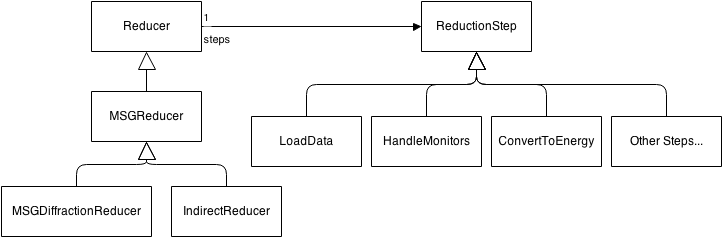
\includegraphics[width=1\textwidth]{img/uml/class_diagrams/Reducer_structure.png}
\caption{Diagram showing the class structure for the inelastic reducers and accompanying reduction steps.}
\label{fig:reducer-structure-diagram}
\end{figure}

Figure \ref{fig:reducer-structure-diagram} shows the class structure of indirect reducers and a subset of the reduction steps that are defined for indirect energy reduction. In indirect data analysis we have two concrete reducer objects. One for energy conversion (IndirectReducer) and one for diffraction reduction (MSGDiffractionReduction). This section will just focus on the IndirectReducer. For discussion on diffraction reduction see section \ref{subsec:indirect-diffraction}.

The IndirectReducer object defines what steps should be executed as part of a reduction work-flow and is the point at which the parameters gather from the user interface are passed to the program. After setting up the each reduction step with the relevant parameters, the reducer then iterates over the list of steps and executes each one in turn on the sample run to be reduced. Reducer objects also have the option to define a preprocessing function which is only executed once regardless of the number of runs being processed. The MSGReducer, which is the superclass of both the IndirectReducer and the MSGDiffractionReducer, uses this to execute the loading step to get the sample run(s) to be reduced into memory before continuing with the rest of the reduction on a per run basis.

\begin{figure}[H]
\centering
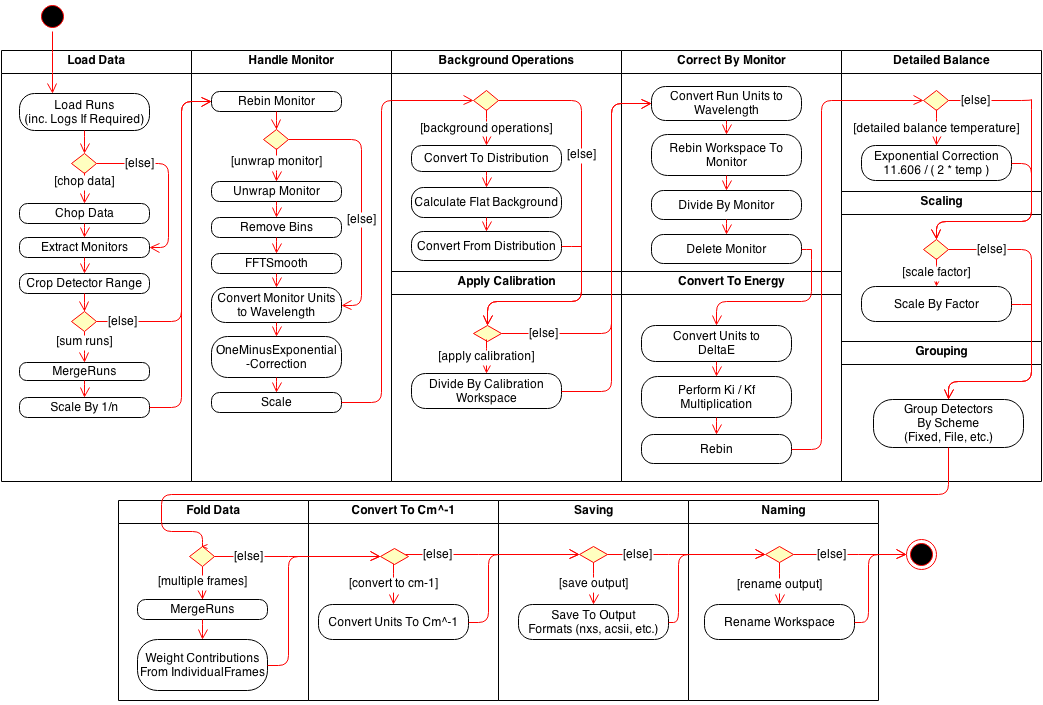
\includegraphics[width=1\textwidth]{img/uml/activity_diagrams/EnergyTransfer_activity.png}
\caption{Activity diagram showing the flow of execution for energy transfer reduction in release 3.2.}
\label{fig:c2e-energy-transfer-activity-diagram}
\end{figure}

The steps involved in energy transfer reduction are shown in activity diagram \ref{fig:c2e-energy-transfer-activity-diagram} along with the major operations performed within each step and the flow of execution for the reduction. The responsibility of each of the steps are as follows:

\begin{itemize}
\item \textbf{Load Data} - The load data step loads each individual sample run from file using the correct loader for the currently selected instrument. If the option is selected, it will also attempt to load the logs for the runs as well. If the current instrument has the parameter Workflow.ChopDataIfGreaterThan defined  in its instrument parameter file (IPF), the reduction step splits the data into multiple frames using the ChopData algorithm. The routine will then extract the monitor from the loaded workspace and crop the workspace to the desired detector range. If the sum option is checked the runs will be merged into a single workspace and averaged, otherwise subsequent steps are executed on each run individually.

\item \textbf{Handle Monitor} - Next the reducer prepares the monitors for correction in a later step. This involves rebinning the monitor according to the step size defined the IPF. Next it will unwrap the monitor, if required, using the UnwrapMonitors algorithm to convert the workspace to have common bins within the maximum wavelength range given a reference flightpath between source, sample and the first detector. It then tidies up the monitor by removing the bin at the joining wavelength and smooths it Using FFTSmooth. Finally it converts the units of the workspace to wavelength, performs an exponential correction for the thickness, attenuation, and area of the monitor and scales it if a scaling factor is defined in the IPF.

\item \textbf{Background Operations} - This step simply calculates a flat background for the detector data if parameters are defined for the background range by calculating the mean of the bins in this range before dividing by the width of the x range.

\item \textbf{Apply Calibration} - If a calibration file was supplied as a parameter to the reduction, the reducer will divide the workspace by the calibration run at this point. This just uses the standard Mantid Divide algorithm.

\item \textbf{Correct By Monitor} - The reducer then corrects the workspace by the preprocessed monitor by converting the units to wavelength then rebinning it to, then dividing it by, the monitor.

\item \textbf{Convert To Energy} - The conversion of the workspace to units of energy is then performed and multiplied by $k_i / k_f$ , to transform the differential scattering cross section into a dynamic structure factor. The workspace is then rebinned according to the user defined rebin string if one was supplied.

\item \textbf{Detailed Balance} - The detailed balance step performs an exponential correction on the data if a temperature parameter was defined by the user. This uses the ExponentialCorrection algorithm.

\item \textbf{Scaling} - This step will scale the workspace by an arbitrary factor supplied by the user.

\item \textbf{Fold Data} - If the data was split into multiple frames during the loading step, the fold data step is performed. The individual frames are merged back into a single workspace (using the MergRuns algorithm) and the workspace is scaled by averaging the contributions of each individual frame across the x range.

\item \textbf{Convert To $Cm^{-1}$} - If the option was selected, the workspace is converted to units of wavenumber.

\item \textbf{Saving} - If any save options were selected, the reduced workspace is saved in the desired formats to the default save directory.
\item \textbf{Naming} - Finally, the reduced workspace is renamed according to the instrument-analyser-refection convention used in Mantid indirect.
\end{itemize}

Note that the instrument parameters used in energy transfer reduction are defined in files called \seqsplit{\textless instrument\_name\textgreater\_Parameters.xml} and \seqsplit{\textless instrument\_name\textgreater\_\textless analyser\textgreater\_\textless reflection\textgreater\_Parameters.xml} where the instrument name, analyser, and reflection are replaced by the actual values used (e.g. IRIS\_graphite\_002\_Parameters.xml) and are kept in the instrument folder within the Mantid installation directory.

\subsubsection{Calibration}
\label{subsec:c2e-calibration}
The calibration section of the convert to energy interface can be used to create calibration and resolution files using vanadium sample runs which are used as part of data reduction and analysis. Calibration workspaces are generated by creating an executing a single reduction step object  (without creating a reducer object) called CreateCalibrationWorkspace. The procedure for generating a single calibration file is to load the runs, and if there is more then one of them merge them and scale the output workspace by a factor of $1/\,number\,of\,runs$. A flat background is then calculated using the background range supplied by the user. The routine then integrates over the peak range (again, supplied by the user) and scales the resulting workspace by an arbitrary factor. An activity diagram for the routine is shown in figure \ref{fig:c2e-calibration-activity-diagram}.

\begin{figure}[H]
\centering
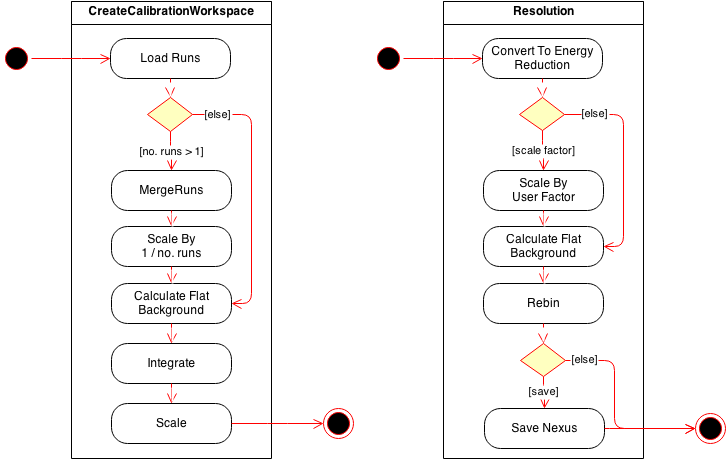
\includegraphics[width=0.6\textwidth]{img/uml/activity_diagrams/Calibration_activity.png}
\caption{Activity diagram showing the major steps of execution performed when creating a calibration and resolution workspace.}
\label{fig:c2e-calibration-activity-diagram}
\end{figure}

As mentioned, the calibration interface can also create resolution files for later use in data analysis. This routine, like many within the indirect code base, is separate from the reducer-reduction step  framework and is just a python function which is executed with parameters supplied from the interface. To create the resolution file, the routine first takes the vanadium run supplied on the calibration interface and converts it to energy using the energy transfer reducer described in section \ref{sec:energy-transfer}, but sets the detector mapping use all detectors and will sum multiple runs if more than one run is used. It then, like calibration, calculates a flat background from a range supplied by the user, rebins it according to the parameters specified for the instrument, and optionally saves the workspace to file in the default save directory.

\subsubsection{Diagnostics}
The diagnostics routine (called Slice in IndirectEnergyConversion.py, named after the older routine from MODES \citep{wshowells2010}) provides an integration over a specified time-of-flight range. The slice routine begins by loading input files and the calibration file if supplied. If a calibration workspace is supplied, it is cropped to remove the monitors and match the range of the input raw file. For each sample workspace input is cropped to the desired number of spectra and divided by the calibration workspace if it exists. The workspace is then integrated across the supplied time range. If two ranges are given, the second range is used to remove a flat background prior to the integration using CalculateFlatBackground. Finally, the resulting workspace is transposed using the algorithm of the same name.

\begin{figure}[H]
\centering
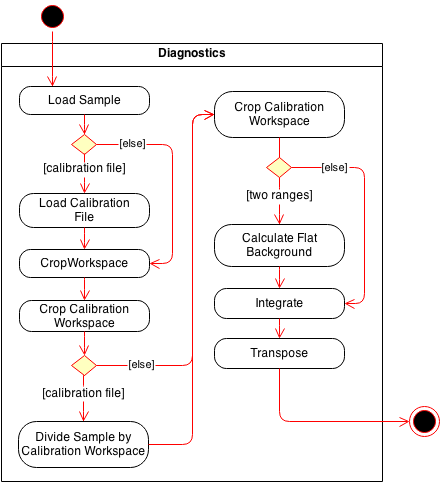
\includegraphics[width=0.5\textwidth]{img/uml/activity_diagrams/Diagnostics_activity.png}
\caption{Activity diagram showing an activity diagram for the Transmission routine.}
\label{fig:c2e-diagnostics-activity-diagram}
\end{figure}

\subsubsection{Transmission}
The transmission routine is a simple program used to calculate the measured transmission of a sample using the incident and transmission monitors. Using a run of both the sample and the can, monitors from each  raw file are extracted and converted to units of wavelength. The transmission monitor is then normalised by the incident monitor in each run over the common wavelength range. Finally, the sample is divided by the can to give the sample transmission as a function of wavelength.

The procedure for doing this using the Mantid API is shown in the activity diagram \ref{fig:c2e-transmission-activity-diagram}. The routine assumes that the first two spectra in a raw file are the monitors (as is generally the case for ISIS indirect instruments) where the first is the incident monitor and the second is the transmission monitor. It also loads the third spectrum in the raw file (which should be actual detector data) to use as a reference time range. 

If the first value on the detector's x-axis matches the corresponding value on the incident monitor it simply converts the monitor workspace to units of wavelength. If it does not match the monitor must first be unwrapped using the UnwrapMonitor algorithm with a hard coded parameter for the flight path of 38.76. Then it corrects the join wavelength for the UnwrapMonitor algorithm by removing the bins at the join with a linear interpolation method that uses the FFTSmooth algorithm for smoothing. It then crops the incident monitor to the shortest wavelength of the two monitors and rebins the second monitor to match. The transmission monitor is then divided by the incident monitor.

\begin{figure}[H]
\centering
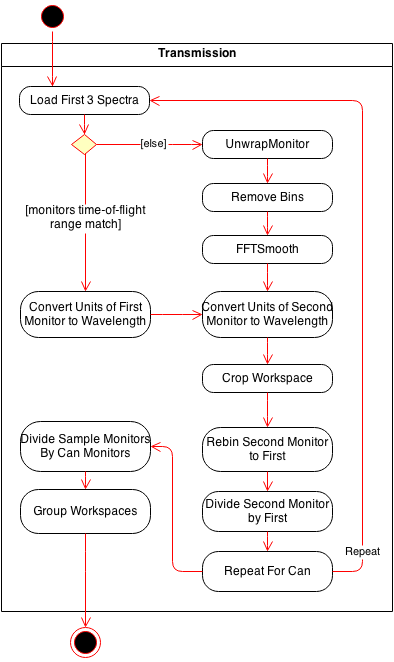
\includegraphics[width=0.4\textwidth]{img/uml/activity_diagrams/Transmission_activity.png}
\caption{Activity diagram showing the flow of execution for the Transmission routine.}
\label{fig:c2e-transmission-activity-diagram}
\end{figure}

This procedure is repeated for both the sample and the can file provided by the user. After the monitors for both the sample and can have been converted the sample transmission monitor is then divided by the can transmission monitor. Finally, a group workspace containing the sample transmission monitor, can transmission monitor, and sample transmission monitor with can removed is created.

\subsubsection{$S(Q,w)$}
\label{subsec:sofqw}
In this interface, reduced files created as part of an energy transfer reduction can be converted to an $S(Q,w)$ workspace. The Mantid framework has a collection of three algorithms that are used to convert a workspace from energy transfer to $S(Q,w)$ depending on the choice of rebinning to use. The mapping between $S(Q,w)$ algorithms and the rebin types are given in table \ref{table:sofqw-algorithms}. The code running an $S(Q,w)$ conversion is entirely contained within the Indirect interface where it dynamically builds a string of python code that is then executed. Optionally, the user many rebin the workspace in energy before hand. In this case, the routine simply calls the rebin algorithm with supplied parameters.

\begin{table}[H]
\begin{center}
\begin{tabular}{ c c}
Rebin Type & Algorithm Used \\ \hline
Centre & SofQW \\
Parallelepiped & SofQW2 \\
Parallelepiped / Fractional Area & SofQW3 \\
\end{tabular}
\caption{Table showing the relationship of rebin types to SofQW algorithms}
\label{table:sofqw-algorithms}
\end{center}
\end{table}

Each the approach to rebinning taken by each of the algorithms listed in table \ref{table:sofqw-algorithms} is as follows:
\begin{itemize}
\item \textbf{SofQW} - The simplest version of the algorithm iterates over each individual detector in a workspace with units of energy transfer and calculates the value of Q using parameters from the instrument and detector and rebins by using the centre point of the bin between two points in the workspace.
\item \textbf{SofQW2} - This version calculates the width of theta over all detectors and uses the maximum and minimum as the offset for the value of theta in combination two points in energy transfer to define a quadrilateral for rebinning. This algorithm inherits from the Rebin2D algorithm and uses its methods to rebin both axes without the use of the fractional area option.
\item \textbf{SofQW3} - The third version of the algorithm is an extension of the second. Again, this algorithm inherits from Rebin2D but uses the fractional area option to rebin. This algorithm also takes into account the angular width based on each individual detector and in the case of PSDs also accounts for the value of phi.
\end{itemize}

\subsubsection{$S(Q,w)$ Moments}
\begin{figure}[H]
\centering
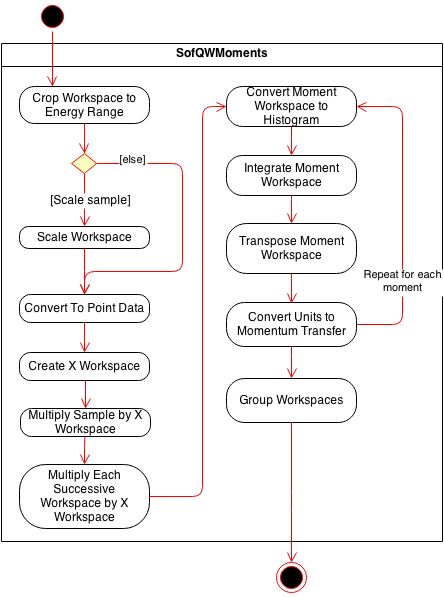
\includegraphics[width=0.4\textwidth]{img/uml/activity_diagrams/SofQWMoments_activity.png}
\caption{Activity diagram showing the flow of execution for the SofQWMoments algorithm.}
\label{fig:c2e-transmission-activity-diagram}
\end{figure}

This is a new addition in Mantid 3.2 and provides a simple routine for calculating the first four statistical moments of an $S(Q,w)$. This is implemented as a standard Mantid algorithm (SofQWMoments) which is created and called from the interface though the algorithm manager and produces a group workspace with one workspace for each moment for every detector which has been transposed in order to make visualisation of the workspace easier.

This algorithm proceeds by first cropping the sample to the desired energy range and optionally scaling it by an arbitrary factor. The sample is then converted from histogram data to point data. A workspace contain the x values of the sample workspace on both axes is then created using the CreateWorkspace algorithm. The sample workspace is then multiplied by this workspace using the Multiply algorithm. The result of this operation is then again multipled by the X workspace. This process repeats on each successive resulting workspace for every moment. These resulting workspaces are then converted back to histogram data, integrated, transposed, and converted to units of momentum transfer. Finally each of the moment workspaces is placed in a single group workspace.

\subsubsection{Support for the ILL}
The convert to energy reduction currently supports instrument at ISIS and the SNS. In release 3.2 a lot of work has been done in order to increase the level of support for ILL instruments. Prior releases of Mantid added a loader for ASCII data files from the ILL to the Indirect Load ASCII interface and stored in the file IndirectNeutron.py. In 3.2 loaders for various ILL instruments (including the very useful LoadILLIndirect) have been added. Additionally, a new reduction algorithm for IN16B, called IndirectILLReduction, has been to give support for energy transfer reduction within Mantid. Future releases aim to integrate this algorithm into the current reduction chain and therefore completely remove Indirect Load ASCII from the system.

\subsection{Diffraction Reduction}
\label{subsec:indirect-diffraction}
Another key part of data reduction is the ability to reduce diffraction data. The process of preparing diffraction runs for analysis is much simpler than an energy transfer reduction. Indirect diffraction reduction uses the same reducer system as described in section \ref{sec:energy-transfer} but uses the MSGDiffractionReducer object (see figure \ref{fig:reducer-structure-diagram}) and a different selection of reduction steps. 

The instrument parameters used in reduction are defined in files called \seqsplit{ \textit{\textless instrument\_name\textgreater}\_diffraction\_diff\_spec\_Parameters.xml} and \seqsplit{ \textit{\textless instrument\_name\textgreater}\_diffraction\_diff\_only\_Parameters.xml} (if the instrument supports diff only mode).

\begin{figure}[H]
\centering
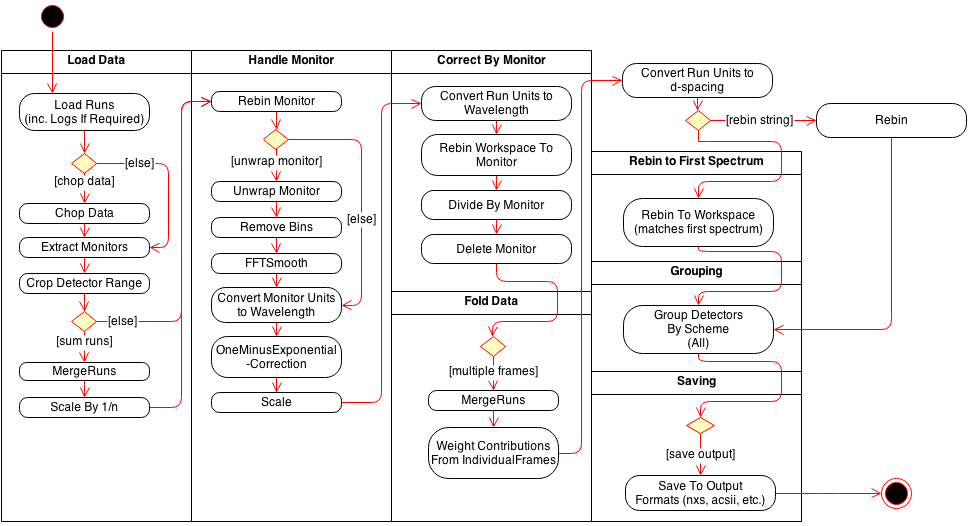
\includegraphics[width=0.9\textwidth]{img/uml/activity_diagrams/DiffractionReduction_activity.png}
\caption{Activity diagram showing the flow of the Diffraction Reduction in release 3.2. Steps outside of boxes are individual algorithms that are not part of a reduction step.}
\label{fig:diffraction-class-diagram}
\end{figure}

\begin{itemize}
\item \textbf{Load Data} - The first step in diffraction reduction is to load all of the data files to be reduced. This reduction step is exactly the same as the one described in section \ref{sec:energy-transfer}.

\item \textbf{Handle Monitor} - Next the reducer prepares the monitors for correction. Again the procedure for this step is exactly the same as the one described in section \ref{sec:energy-transfer}.

\item \textbf{Correct By Monitor} - Again this is the same as described in section \ref{sec:energy-transfer}, but when running the convert units algorithm to convert the workspace to wavelength the reduction step uses the Elastic energy mode option instead of Indirect energy mode option.

\item \textbf{Fold Data} - If the data was split into multiple frames during the loading step, the fold data step is performed. This is identical to the step described in section \ref{sec:energy-transfer}.

\item \textbf{Convert Units To $d$-spacing} - This is not a reduction step, but just a call to the Mantid ConvertUnits algorithm to covert the workspace to units of $d$-spacing with the energy mode used being elastic.

\item \textbf{Rebin} - If the a rebin string was supplied to the reducer, the workspace is rebinned according to the supplied parameters. Again this is not a reduction step but just a plain call to the Rebin . If no rebin string was supplied, the workspace is rebinned to the first spectrum using the reduction step of the same name. This step just calls the RebinToWorkspace algorithm with all arguments set to the same workspace.

\item \textbf{Grouping} - Next the grouping reduction step is performed, which is the same as in section \ref{sec:energy-transfer} but with the grouping type hard coded to simply show all spectra.

\item \textbf{SaveItem} - Finally, the reduced workspace is past through the SaveItem reduction step where the output options past to the reducer are processed. Once again, this step is identical to the one described in section \ref{sec:energy-transfer}.

\end{itemize}

The OSIRIS instrument can double as a diffractometer with a much larger diffraction detector range compared to the other indirect instruments at ISIS. It therefore uses a specialised algorithm called OSIRISDiffractionReduction for use in diff only mode and does not use the reducer chain. OSIRISDiffractionReduction is based off of the ARIEL program \citep{pradaelli2000ariel}. 

This algorithm takes a list of samples and a list of vanadium runs and an old style calibration file (these are not the ones generated by the routine in section \ref{subsec:c2e-calibration}, but the type supplied to the AlignDetectors and DiffractionFocussing algorithms). Each of the sample/vanadium run pairs can cover a different $d$-range which the algorithm then merges using the MergeRuns algorithm. This algorithm proceeds as follows:

\begin{figure}[H]
\centering
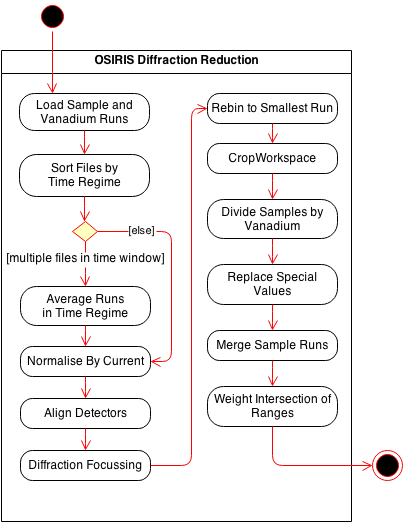
\includegraphics[width=0.4\textwidth]{img/uml/activity_diagrams/OSIRISDiffractionReduction_activity.png}
\caption{Activity diagram showing the flow of the OSIRIS Diffraction Reduction in release 3.2.}
\label{fig:OSIRISdiffraction-class-diagram}
\end{figure}

\begin{itemize}
\item The algorithm begins by loading all of the samples and vanadium runs into workspaces. This just uses the standard Load algorithm.

\item The algorithm then maps each of the supplied samples to there corresponding $d$-range and averages any workspaces that are in the same $d$-range. The same procedure is repeated for the vanadium runs.

\item If multiple runs or Vanadium samples have been supplied for the same time regime the algorithm will take the average of all samples/Vanadium runs in the time regime. This just uses the Mantid Plus and Divide algorithms to calculate the mean of the workspaces. 

\item At this point the algorithm has a processed list of all workspaces and their background for each $d$-range and can begin the reduction. The algorithm now normalises by the beam current, aligns detectors, and performs diffraction focussing using the calibration file provided. It then crops the workspace to match it's $d$-range. These operations are performed for each sample and vanadium run.

\item The background for the runs is then processed by rebinning each sample/vanadium pair to match the smallest of the pair (using the RebinToWorkspace algorithm) and then divides the sample by the vanadium. Any NaN or infinity values after this operation are replaced with zeros using the ReplaceSpecialValues algorithm.

\item Finally all of the samples are merged into a single workspace using the MergeRuns algorithm and the workspace is weighted at the points of intersection where the ranges overlap by scaling by the number of overlapping contributions at a given point.
\end{itemize}

\subsection{Data Reduction GUI}

\subsubsection{Energy Transfer GUI Overview}
\label{subsec:c2e-gui-overview}
Figure \ref{fig:c2e-class-diagram} shows the class structure of the indirect convert to energy. Note that for clarity only a selection of the more fundermental methods and attributes are shown as part of the class diagram. The Convert to Energy window (for both direct and indirect instruments) inherits from Mantid's generic UserSubWindow class which provides the basic functionality required to render a sub window within the application and also provides some useful helper methods such as the ability to execute a string as a python script.

The ConvertToEnergy class itself contains the code which is shared between both direct and indirect versions of the interface. It is responsible for the loading the appropriate instrument definition files as the user selects an instrument, swapping between the indirect and direct interfaces depending on the geometry of the selected instrument, and handling the major user actions such as clicking the run energy transfer and help buttons.

\begin{figure}[H]
\centering
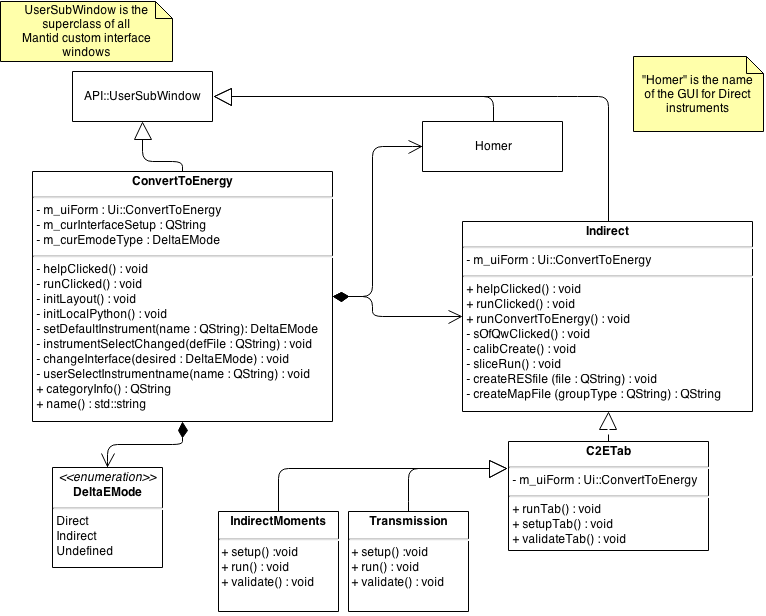
\includegraphics[width=0.8\textwidth]{img/uml/class_diagrams/C2E_structure.png}
\caption{Class diagram showing the structure of the Indirect Convert To Energy GUI in release 3.2.}
\label{fig:c2e-class-diagram}
\end{figure}

ConvertToEnergy is composed with two classes called Homer and Indirect that handle the functionality of direct and indirect geometry instruments respectively. In previous releases of Mantid the Indirect class contained all of the GUI code for every tab on the Indirect Convert To Energy interface. This is no longer the case in more recent versions of Mantid which have moved towards a more modular class structure.

As of release 3.2, the Indirect class contains the GUI code for the Energy Transfer, Calibration, Diagnostics, $S(\textbf{Q},w)$, and Moments tabs. For each of these tabs there are corresponding methods (which are inconsistently named) to validate the user's input for that tab and run the appropriate routine. The specifics of each of these routines is outlined in the following sections. In order the execute the required routine, the GUI code for a particular tab builds a string which represents an executable python script complete with the options collected from the interface that can be executed using the runPythonCode() method inherited from UserSubWindow.

The actual design of the GUI is stored in a separate xml file that was created using Qt Designer and is used to produce a dynamically generated class for the interface at compile time which includes all the interface widgets for ConvertToEnergy. The ConvertToEnergy, Homer, and Indirect classes each have a reference to a copy of this interface object which they can query at runtime. The ConvertToEnergy class is responsible for adding and removing the appropriate tabs as the user switches between instrument geometries. The Indirect class uses this reference to query user input and update the interface appropriately in response to user actions.

In the past year there have been two additional tabs added to the Convert To Energy interface which do not follow the monolithic class structure currently used by the majority of tabs in the indirect energy conversion interface. Instead of adding the code for the additional tabs IndirectMoments and Transmission directly into the Indirect class, a new class was created called C2ETab which is composed with the Indirect class (see diagram \ref{fig:c2e-class-diagram}). The specific implementations of the two new tabs are then handled by a specific class derived from the abstract C2ETab.

This approach is similar to the one already place in the Indirect Data Analysis interface (see \ref{subsubsec:IDA-GUI-Overview}) and provides a number of benefits over the initial design. Structuring the code in this way allows for greater modularity because each subclass of C2ETab is only concerned with the functionality relating to a single tab on the interface.

Furthermore, this design still allows code that is common between multiple tabs (such as code for plotting a histogram in a mini-plot) to be written once and shared across all classes through inheritance. Note that C2ETab also has a reference to the UI object so that it can interact with the widget objects defined on the interface, however this could easily be changed to use tab orientated interface objects (like the approach used by IndirectBayes, see \ref{subsubsec:Bayes-GUI-Overview} and further discussion in \ref{subsec:GUI-Improvements}) instead of having unrestricted access to the whole interface.

\subsubsection{Indirect Diffraction GUI Overview}
The corresponding interface for diffraction reduction is called Indirect Diffraction. Unlike the other interfaces in the Indirect collection, the structure of this interface is just a single class with a single UI file defining the layout. Each instrument has either the option of running in diff spec or diff only mode (TOSCA and VESUVIO only have diff spec mode) and, as described in the previous section, OSIRIS has a different reduction routine in the case of diff only mode. This is reflected in the interface when the user selects the appropriate option. The GUI changes the way the interface looks by checking the instrument parameter files for the currently selected instrument and reflection.

\subsection{An Example Reduction}
In this final subsection, we illustrate an example reduction of some data from the IRIS instrument using the Indirect Convert To Energy GUI in Mantid. The screen shot in figure \ref{fig:iris-c2e-reduction} shows the Indirect Convert to Energy interface in release 3.2. The example shows the instrument selected as being IRIS and using the graphite analyser with reflection 002. One or more runs can be selected using the file browser in the input files section of the interface.

\begin{figure}[H]
\centering
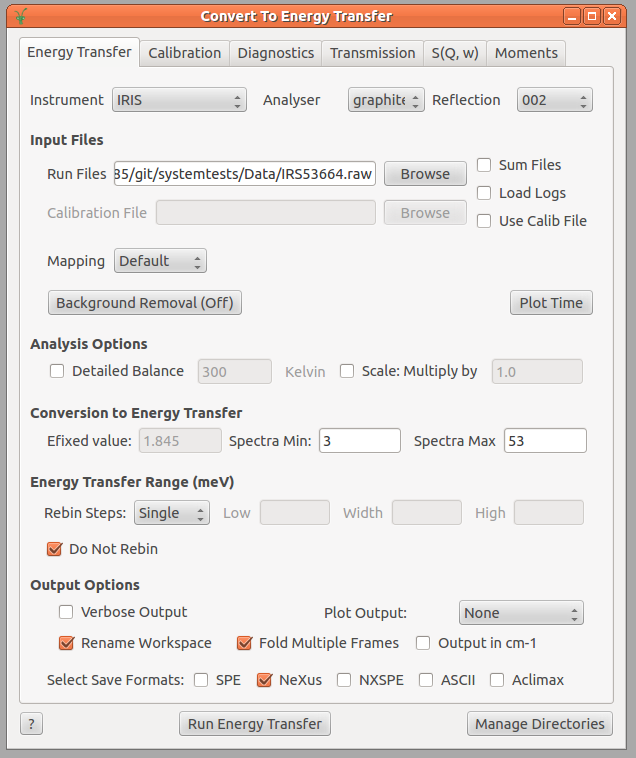
\includegraphics[width=0.5\textwidth]{img/iris-c2e-reduction.png}
\caption{Indirect Convert to Energy interface reducing some data from the IRIS instrument in release 3.2}
\label{fig:iris-c2e-reduction}
\end{figure}

There are lots of additional options that can be configured depending on the users requirements for the output of the reduction. This includes the rebinning, spectrum mapping, and detector ranges to be used, whether to sum the files and what formats to save the resulting workspace as (in the user's default save directory). All of these options are set to a sensible default for each instrument as it is selected, so in the simplest case all the user needs to do is select there instrument and the appropriate run file(s) and click run energy transfer.

\begin{figure}[H]
\centering
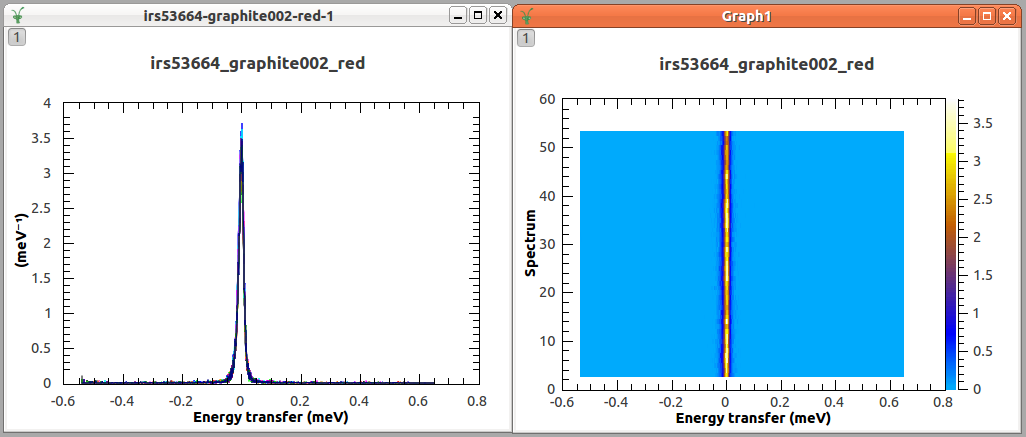
\includegraphics[width=0.8\textwidth]{img/iris-c2e-reduction-plot.png}
\caption{Reduced IRIS data plotted as both a contour and spectrum plot}
\label{fig:iris-c2e-reduction}
\end{figure}

Doing this with the settings shown in figure \ref{fig:iris-c2e-reduction} produces a single workspace for run 553664 on the IRIS instrument with units of energy transfer. This workspace can then be used with the Indirect Data Analysis and Indirect Bayes interfaces. We can also run this through the SofQW algorithm to calculate the $S(\mathbf{Q},\omega)$ and convert the workspace to units of momentum transfer using the SofQW tab on same interface.

\begin{figure}[H]
\centering
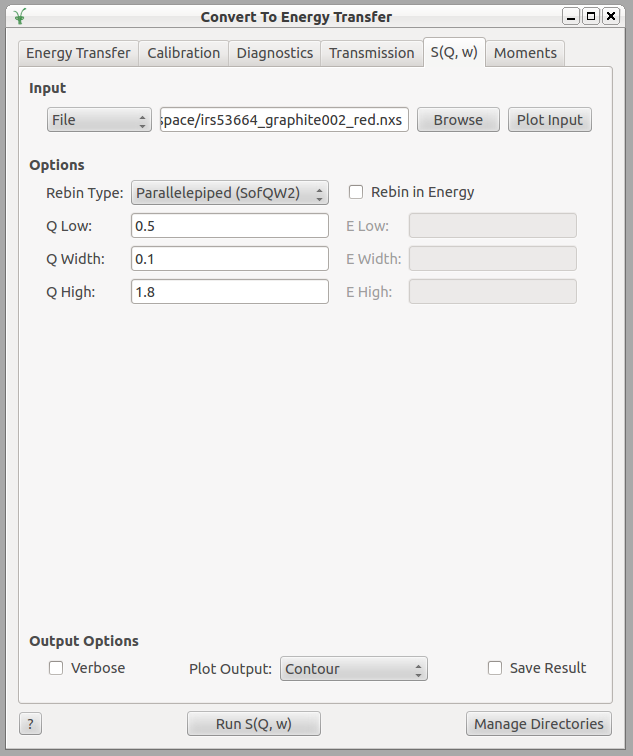
\includegraphics[width=0.5\textwidth]{img/iris-c2e-sofqw.png}
\caption{Indirect Convert to Energy interface converting some reduced data output from the previous screen shot using the SofQW algorithm  in release 3.2}
\label{fig:iris-c2e-sofqw}
\end{figure}

This interface allows us to specify the binning we use in Q and in energy and also the type of rebinning to be used in the conversion (see section \ref{subsec:sofqw}). Plotting the resulting \*\_sqw workspace as a contour plot shows energy transfer vs. Q.

\begin{figure}[H]
\centering
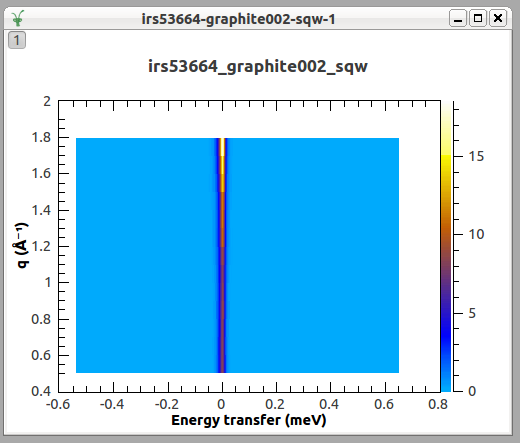
\includegraphics[width=0.5\textwidth]{img/iris-c2e-sofqw-plot.png}
\caption{Contour plot of a \*\_sqw workspace in release 3.2}
\label{fig:iris-c2e-sofqw-plot}
\end{figure}

\section{Data Analysis with Mantid}

After data has been reduced using the convert to energy or diffraction reduction routines described in the previous section the reduced data needs to be analysed. In the indirect section of Mantid, there are two major collections of data analysis scripts that are currently in place. The first  and most important are those included in the Indirect Data Analysis interface which provide a variety of different fit functions and transforms the can be performed on reduced data. The second collection of routines are accessible via the Indirect Bayes interface. This provides a collection of routines that can be used to infer fitting parameters using Bayesian model selection techniques which are complementary to the routines in Indirect Data Analysis.

The majority of the code for data analysis scripts can be found in the file IndirectDataAnalysis.py with the Inelastic script folder of the Mantid installation, with the exception of Calculate Corrections which is in a file called IndirectAbsCor.py. For the Bayesian fitting programs, the code is stored in the file IndirectBayes.py, with the exception of JumpFit which is stored in IndirectJumpFit.py both of which are in the Inelastic scripts folder.

\subsection{Basic Analysis}
\subsubsection{ElWin}
The ElWin (elastic window) program is used to perform elastic window scans by integrating over the energy range of a reduced file and is based on the routine of the same name that was originally provided as part of the MODES package \citep{wshowells2010}. As with most all routines in the Indirect Data Analysis interface, the ElWin is implemented as a collection of free standing functions in IndirectDataAnalysis.py. Internally, this routine uses Mantid's ElasticWindow algorithm. This a small C++ side algorithm that integrates over the input workspace. The script provided in IndirectInelastic.py pre and post processes the data. 

The elastic window algorithm converts the spectrum axis of the input workspace to two output workspaces with units of $Q$ and $Q^2$. Both of these workspaces are then transposed so they are easier to visualise. Optionally, this routine can also remove a background using a second range. The $Q^2$ output for ElWin is used as the input to the MSDFit routine described in the following section.

\begin{figure}[H]
\centering
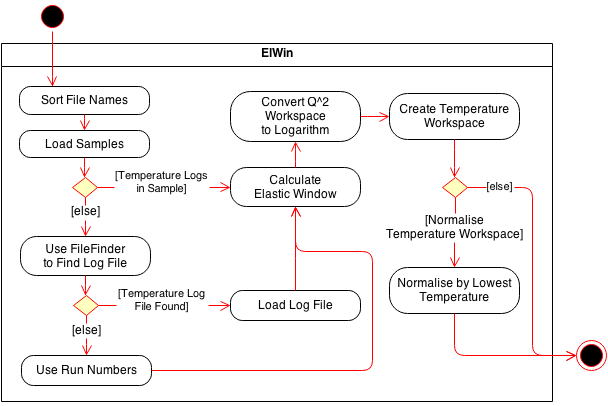
\includegraphics[width=0.6\textwidth]{img/uml/activity_diagrams/ElWin_activity.png}
\caption{Activity diagram for the ElWin routine.}
\label{fig:elwin-acticity-diagram}
\end{figure}

The ElWin routine proceeds by first sorting the list of workspace names supplied as input. As there is an unofficial naming convention in the indirect inelastic section of Mantid where the names include the run number, this should produce a list with the smallest run number first.

The program then iterates over each workspace and attempts to extract temperature information from the sample logs. The logs will only be present if the Load Logs option was checked during an energy transfer reduction. Otherwise, the routine searches the users managed directories for a log file matching the log number and name of the instrument for the current run and loads it using the LoadLog algorithm. If no logs are found then the run numbers for each file are used instead of temperature.

The ElasticWindow algorithm is then executed on the sample. Optionally two ranges can be supplied which will remove a flat background from the workspace first. The algorithm produces the two workspaces in units of Q and $Q^2$. The $Q^2$ workspace is then converted to be the Logarithm of the data.

Finally, a third workspace is created from the two output from the ElasticWindow algorithm with units of Kelvin on the x axis vs. momentum transfer on the y axis. This uses the value for temperature loaded from the sample logs at the start of the routine. If the option is selected, the temperature workspace is normalised by the lowest temperature in the workspace.

\subsubsection{MSDFit}
\label{subsubsec:msdfit}

\begin{figure}[H]
\centering
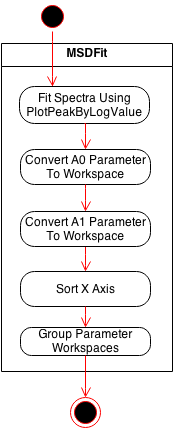
\includegraphics[width=0.2\textwidth]{img/uml/activity_diagrams/MSDFit_activity.png}
\caption{Activity diagram for the MSDFit routine.}
\label{fig:msdfit-acticity-diagram}
\end{figure}

The MSD fit routine is used to calculate the mean squared displacement from the $Q^2$ workspace output from ElWin. In essence this routine performs a linear fit to every spectrum in the workspace using the algorithm PlotPeakByLogValue. However the routine also performs some additional operations to transform the fit parameters from a table workspace to a matrix workspace using the ConvertTableToMatrixWorkspace algorithm. The final parameter workspaces are then grouped.

This routine produces a group workspace contain the linear fits to each spectrum and a workspace for each of the parameters of the fit to each spectrum transposed into a matrix workspace.

\subsubsection{Fury}
The Fury program is used to perform a fast Fourier transform on a reduced workspace in order to calculate the intermediate scattering function $I(Q,t)$. The routine can handle converting multiple workspaces at once, but is currently only set-up to handle the interface to convert one reduced sample at a time.

\begin{figure}[H]
\centering
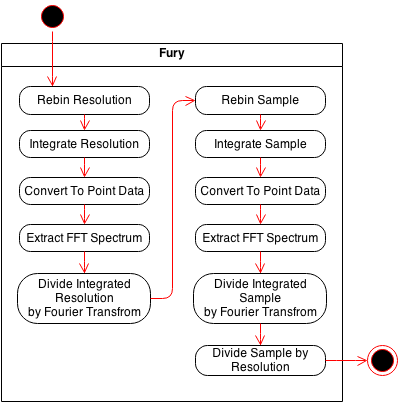
\includegraphics[width=0.4\textwidth]{img/uml/activity_diagrams/Fury_activity.png}
\caption{Activity diagram for the Fury routine.}
\label{fig:fury-activity-diagram}
\end{figure}


The routine first Fourier transforms the resolution workspace then transforms each of the samples using the exact same method and  then divides each of them by the resolution. In order to convert to the intermediate scattering function all of the workspaces must have the same x range and the same regular binning in order for the conversion to work. Therefore the rebin parameters provided by the user must satisfy these conditions. The workspace is then integrated to a separate workspace. The original workspace is then converted to point data in preparation for running the fast Fourier transform algorithm.

The algorithm used is called ExtractFTTSpectrum which runs Mantid's FFT algorithm to on each spectrum in the workspace which outputs the modulus positive frequencies of the transform in the corresponding spectrum. The transformed sample workspaces are then divided by the transformed resolution workspace. The upper half of the transform is then crop off of the workspace to get rid of excess noise from the transform and then optionally saved to a nexus file.

\subsubsection{FuryFit}

\begin{figure}[H]
\centering
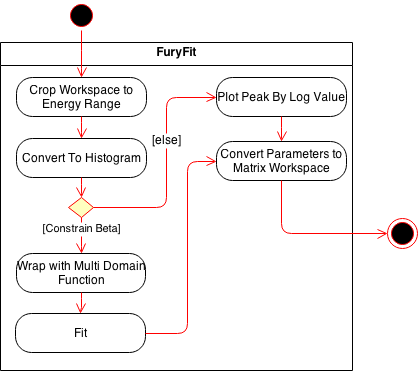
\includegraphics[width=0.4\textwidth]{img/uml/activity_diagrams/FuryFit_activity.png}
\caption{Activity diagram for the Fury Fit routine.}
\label{fig:fury-fit-activity-diagram}
\end{figure}

FuryFit provides a fit routine for the output of Fury offering a variety of decaying exponential functions. Similarly to MSDFit, the routine uses the Fit and PlotPeakByLogValue algorithms to sequentially fit each spectrum with the parameters.

The FuryFit code actually consists of two routines which are very similar and which could be merged in future release of Mantid called FuryFitSeq and FuryFitMult which perform a sequential fit and a multi domain fit respectively. Both routines works by executing a function string which is dynamically created in the GUI code for FuryFit, but FuryFitMult first wraps the input function with a MultiDomain composite function. FuryFitMult is only executed when the user has chosen to constrain the $\beta$ parameter for a stretched exponential fit across all $Q$.

Both of these routines convert the table of fitting parameters created from Fit (or PlotPeakByLogValue) into a matrix workspace using the same code as used by MSDFit.

\subsubsection{ConvFit}
\label{subsubsec:convfit}

\begin{figure}[H]
\centering
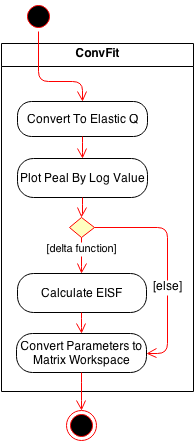
\includegraphics[width=0.2\textwidth]{img/uml/activity_diagrams/ConvFit_activity.png}
\caption{Activity diagram for the Conv Fit routine.}
\label{fig:conv-fit-activity-diagram}
\end{figure}

The ConvFit routine is used to perform a convolution fit to the workspaces. Again, this routine follows a similar procedure to both the MSDFit and FuryFit routines. A fit function with the options the user has selected are gathered from the user interface and a string representing the function to be fitted is passed to the PlotPeakByLogValue algorithm to perform a sequential fit.

The functions fitted are a $\delta$-function, one or two Lorentzians or a combination of both which are then convolved with the user supplied resolution workspace. The type of background can also be selected from a choice of Fixed Flat (flat background without the intercept tied to the user supplied value), Fit Flat (flat background with the intercept unconstrained), and Fit Linear (unconstrained linear background). Optionally a temperature correction can be applied to the Lorentzians. The temperature correction is defined as:

\begin{equation}
f(x) = (\frac{x \cdot 11.606}{t}) / [1 - exp(-\frac{x \cdot 11.606}{t})]
\end{equation}

Where $t$ is the user supplied value for the temperature in kelvin, $x$ is the value in energy transfer at a given point in the workspace and 11.606 is the conversion factor from units of meV to K. Each Lorentzian is multiplied by this factor then convolved with the resolution.

The final composite function is represented as a string that the Mantid fit algorithm can interpret. This function string is generated within the GUI code for ConvFit and then passed to the underlying python routine.

As with the other FuryFit, ConvFit will convert the input workspace to elastic $Q$ first before performing the fit, and converts the output table of fit parameters to a matrix workspace. If a $\delta$-function was used the elastic incoherent structure factor (EISF) is calculated from the resulting table of parameters.

\subsubsection{Calculate Corrections}
Calculate Corrections is used to create a group workspace of absorption corrections from known parameters of the sample and can used in an experiment which can be applied to a reduced workspace using the Apply Corrections routine (see section \ref{subsubsec:apply-corrections}). This routine supports both flat plate and cylindrical geometries.

The code for calculating corrections for a cylindrical geometry is has been ported into Mantid using the F2Py package directly from it's previous incarnation as the Acorn routine in the MODES package. This allows a python script run the Fortran code without it being converted to python code. Unfortunately the downside to this is that F2Py cannot be packaged into the installer for any platform outside of Windows. The code for flat plate corrections was ported in Mantid as part of release 3.2.

In depth discussion on the exact methods of calculating the absorption factors for flat plate and cylindrical geometries can be found in Carlile \citep{ccarlile1974} and the ATLAS manual \citep{aksoper1989} respectively.

The python code underlying the interface of calculate corrections and responsible for liaising between the Fortran and C++ GUI code is (unlike the other routines described in this section) stored in a separate file called IndirectAbsCor.py. This is to keep F2Py import call separate from the rest of the data analysis code, so the other interfaces can be used on platforms other than Windows.

Regardless of the geometry used, the Python/Fortran code calculates four arrays for each spectrum in the sample workspace each of which are collected into four resulting output workspaces with the suffixes \textit{ass}, \textit{assc}, \textit{acsc}, and \textit{acc} which loosely corresponds to the formalism described in Paalman and Pings \citep{hhpaalman1962}. These stand for:

\begin{itemize}
\item \textbf{Ass} - Attenuation factor for scattering in the sample and attenuation in the sample.
\item \textbf{Assc} - Attenuation factor for scattering in the sample and attenuation in the sample plus container.
\item \textbf{Acsc} - Attenuation factor for scattering in the container and attenuation in the sample plus container.
\item \textbf{Acc} - Attenuation factor for scattering in the container and attenuation in the container.
\end{itemize}

If a workspace representing the container is not supplied by the user, then all workspaces except the \**\_ass workspace will just contain zeros.

\subsubsection{Apply Corrections}
\label{subsubsec:apply-corrections}

Apply Corrections provides a complementary routine to the calculate corrections routine described in the preceding section. Apply corrections has two modes of applying corrections to a sample. The first and simplest method is to just take a run of the container for the sample and subtract it from the sample itself. The second uses the corrections workspace generated by the calculate corrections routine and applies them to the sample \& can workspaces (if a can is supplied). A detailed activity diagram of the two modes of execution are shown in diagram \ref{fig:applycorr-activity-diagram}

\begin{figure}[H]
\centering
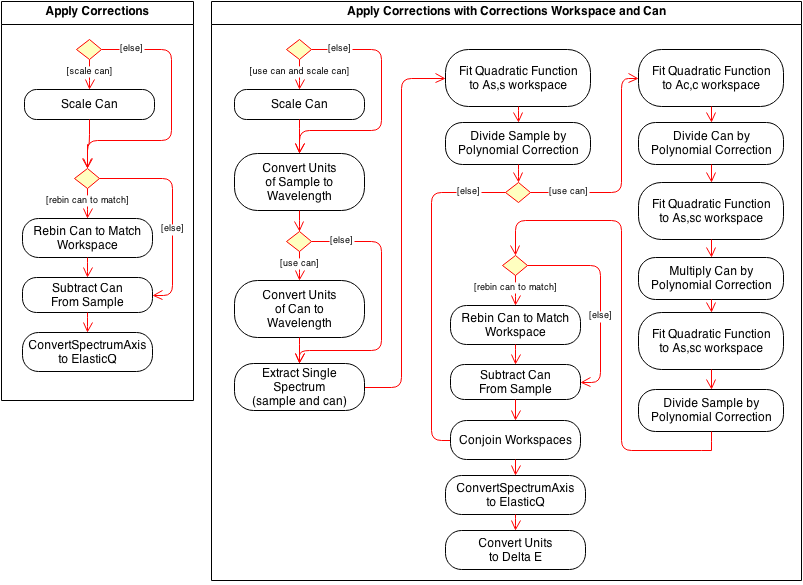
\includegraphics[width=0.8\textwidth]{img/uml/activity_diagrams/ApplyCorr_activity.png}
\caption{Activity diagram showing the flow of the apply corrections routine in release 3.2.}
\label{fig:applycorr-activity-diagram}
\end{figure}

In the former mode of operation (left activity diagram) the scale is first optionally scaled by an arbitrary factor. If the energy ranges of the sample and container do not match the can is rebinned if the user has specified the rebin can option, otherwise an error is thrown. If rebinning the can to match the sample is requested the routine uses the RebinToWorkspace algorithm. After the sample has been corrected, it will use the ConvertSpectrumAxis algorithm to convert the resulting corrected sample to units elastic Q.

In the latter mode of operation, the routine first converts both the sample and container to units of wavelength. Then for spectrum in the sample and can (if supplied), perform a quadratic fit (using the standard Mantid Fit algorithm) to the corresponding spectrum in each of the members of the group workspace of absorption corrections. The coefficients from this fit are then supplied as parameters to the PolynomialCorrection algorithm. The resulting single spectrum workspace for the can is the subtracted from the corresponding single spectrum sample workspace and the result is stitched back together into a single workspace using the ConjoinWorkspaces algorithm. The resulting workspace is output both in units of energy transfer and elastic Q.


\subsection{Advanced Analysis}

The Indirect Bayes interface provides a collection of routines for performing model and parameter selection using Bayesian methods. These routines are, like those in proceeding sections, based on previous implementations in the MODES package. The ResNorm, Quasi, and Stretch routines described in the following sections are all imported into Mantid using the F2Py package directly from the original Fortran code. 

In future releases of Mantid it is hoped that these routines will be converted into proper C++ or Python algorithms as is the case with the rest of Mantid. The routines defined in here are included in Mantid in the file IndirectBayes.py and the accompanying Fortran modules which are in the same folder. The majority of the code in this file does not currently use standard Mantid algorithms, largely because the the Fortran code obviously doesn't work with workspaces and so we are reduced to working with numpy arrays and manually building workspaces. Worse than this, in the Quasi fitting routine the fit parameters get written to file, which is then immediately read back into the program which is both unnecessary and hugely inefficient.

\subsubsection{ResNorm}
ResNorm is used to create a group normalisation workspace which can be input to the Quasi routine (described in the next section). It normalises the input data using the instrument resolution by fitting. A group normalisation may also be done by grouping Q values where the resolution is stretched using a stretch factor. The routine produces two group workspaces with the suffixes \**\_ResNorm and \**\_ResNorm\_Fit respectively. The ResNorm group workspace contains two workspaces with the suffixes intensity and stretch. The intensity workspace contains the intensity normalisation factor and stretch contains a stretch factor for the width of the supplied resolution file. The ResNorm\_Fit group workspace contains the fits to each spectrum in the workspace.

\subsubsection{Quasi}
The Quasi routine provides a model selection algorithm using Bayesian methods to choose the number of lorentzian components present in the input data \citep{dssivia1992} and was originally known as Quasi Lines in the old MODES package \citep{wshowells2010}. This routine takes a sample to fit to and a resolution file created in the convert to energy interface and optionally a resolution normalisation file created in ResNorm (see the previous section). This program can run either by fitting a $\delta$-function plus a sum of Lorentzians or a single stretched exponential.

There are three Fortran modules used depending on the input. The QLres module fits a sum of Lorentzians. If the resolution file contains more than one spectrum, then the QLdata module is used and any ResNorm file supplied is ignored. Finally if the choice of fitting a stretched exponential is used the QLse module is used. Each of these modules share very similar code which is duplicated and modified slightly to suit the specifics of the implementation.

Inside the fitting routine it first refines the parameters for the $\delta$-function, linear background, energy range offset and thereby estimates the probability of the absence of quasielastic components in data. It then refines the parameters for one, two and three Lorentzian components successively \citep{dssivia1992}.

Internally the program loads both the ResNorm and width files into 1D arrays. It then extracts from the sample and resolution workspaces a the x, y, and e arrays for each spectrum in the workspace and passes this data to the Fortran routine with any accompanying fit parameters used. The corresponding fits to the data are returned in the form of x, y, and e arrays for the spectrum and its log probability for each Lorentzian (from 0 to 3). Additionally, the program also reads the program parameters from the generated file (saved in the user's default save directory) and creates a workspace of fit parameters similar to the one output by ConvFit. Likewise, it will also calculate the EISF from the fit parameters.

\subsubsection{Stretch}
\label{subsec:stretch}
Stretch is a variation on the stretched exponential option provided by the Quasi program described in the previous section and was originally called Quest in the old MODES package \citep{wshowells2010}. The Fortran module used is called Que. The operation of the two programs are essentially the same, except that a grid of $\beta$ and $\sigma$ parameters are fitted to each spectrum instead.

This fit routine produces one group workspace containing the fit to the data for each spectrum and two additional workspaces containing the parameters $\beta$ and $\sigma$ parameters of the fit.

\subsubsection{JumpFit}
\label{subsec:jumpfit}
JumpFit provides very simple routine for fitting the width parameters for each spectrum fitted from either the Quasi or ConvFit routines. It offers a collection of diffusion fit functions (defined as Mantid fit functions). The desired component width and function type is selected by the user and a fit function string is built and passed to the Mantid's Fit function. The fit functions used in JumpFit are currently hard coded to use the default values shown in table \ref{table:jumpfit-functions}.

\begin{table}[H]
\begin{center}
\begin{tabular}{ l l l}
Function & Function Definition & Default Parameter Values \\ \hline
Chudley-Elliot &  $\Gamma(Q) = (1 - sin(Ql)/Ql)/\tau$ & $\tau = 1.0/QMax, L=1.5$\\ \hline
Hall-Ross & $\Gamma(Q) = (1-exp(-lQ^2))/\tau$ & $\tau = 1.0/QMax, L=1.5$ \\ \hline
Fick & \parbox{6cm}{$\Gamma(Q) = DQ^2$ \\ where $D=<l^2>/6\tau$} & $D = \Delta y / \Delta x^2$\\ \hline
Teixeira Water & \parbox{6cm}{$\Gamma(Q) = DQ^2/(1 + DQ^2\tau)$ \\ where $D=<l^2>/6\tau$} & $\tau = 1.0/QMax, L=1.5$ \\ \hline
\end{tabular}
\caption{JumpFit function names, definitions, and default parameter values.}
\label{table:jumpfit-functions}
\end{center}
\end{table}

\subsection{TOSCA Data Analysis}
All of the data analysis routines mentioned in the previous section are orientated towards the analysis of quasi-elastic neutron scattering (QENS) data. The TOSCA spectrometer is used to perform inelastic neutron scattering and does not make use of the QENS routines outlined in previous sections. Their data analysis procedures are far simpler. The general process for analysing TOSCA data is to perform an energy transfer reduction as described in section \ref{sec:energy-transfer} and then directly comparing the resulting workspace with one produced from theory using the visualisation tools available through the Mantid framework. Currently the simulated data used in comparison is generated using tools such as Gaussian 03 and a-CLIMAX and then loaded into Mantid. In the future we aim to add more support in Mantid for comparing experimental results with theory (see section \ref{sec:simulation}). As an example, the plot in figure \ref{fig:tosca-analysis} shows a comparison of the experimental result from a sample of toluene with the spectrum generated from theory by simulation programs.

\begin{figure}[H]
\centering
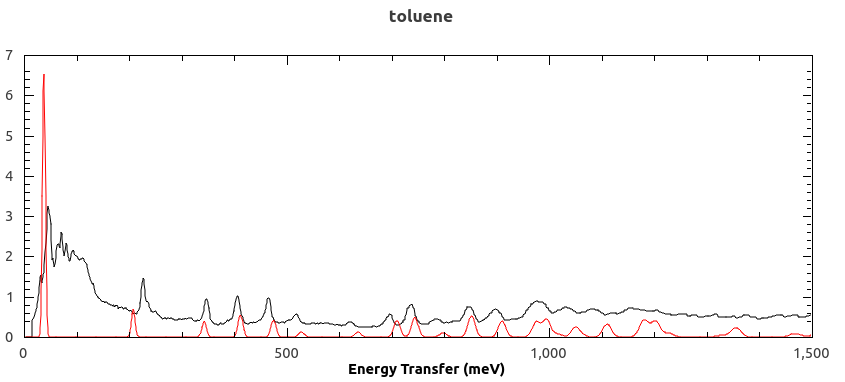
\includegraphics[width=0.7\textwidth]{img/tosca-analysis.png}
\caption{Plot of a toluene sample (run 13930) cooled to 10K in black with theoretical simulation of the spectrum in red.}
\label{fig:tosca-analysis}
\end{figure}


\subsection{VESUVIO Data Analysis}
The VESUVIO spectrometer is currently not officially supported by the Mantid framework. Analysis with the spectrometer is primarily centred on the determination of atomic momentum distributions in condensed matter systems \cite{mayers2012vesuvio}. Development work has already been undertaken to add support for the spectrometer to Mantid. A collection of data analysis routines are available, but are currently under heavy testing and may be unstable. Information on using these routines, how to obtain them, and the progress of development are outlined in Ref. \cite{jackson2014vesuvio}.

\begin{figure}[H]
\centering
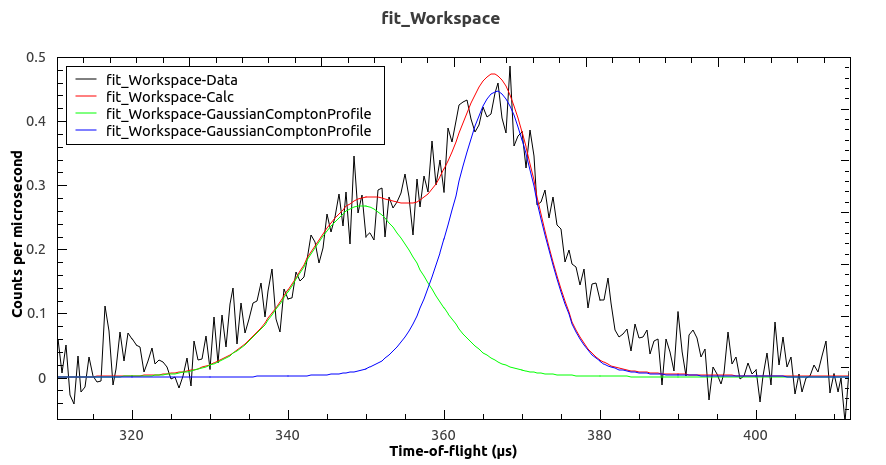
\includegraphics[width=0.7\textwidth]{img/gaussian-fit-example.png}
\caption{Plot of some VESUVIO data for a sample of ZrH$_2$ using the routines described in Ref. \cite{jackson2014vesuvio} and based on the methods described in Ref. \cite{mayers2012vesuvio}. The black line shows the original data, the red line shows the fit to the data is in red, and the individual contributing peaks are in green (aluminium) and blue (zirconium)}
\label{fig:vesuvio-gaussian-fit}
\end{figure}

\subsection{Data Analysis GUI}

\subsubsection{Indirect Data Analysis GUI Overview}
\label{subsubsec:IDA-GUI-Overview}
The Indirect Data Analysis user interface follows a similar design structure to the Convert To Energy interface but is more modular. The interface is composed of a single parent class for the window which sets up and manages all tabs on the interface and is simply called IndirectDataAnalysis. A collection of classes for each tab on the interface which inherit from a common base class, similar to the C2ETab class in the convert to energy GUI, are composed with the window class to handle the specific implementation details of each the corresponding tabs.

\begin{figure}[H]
\centering
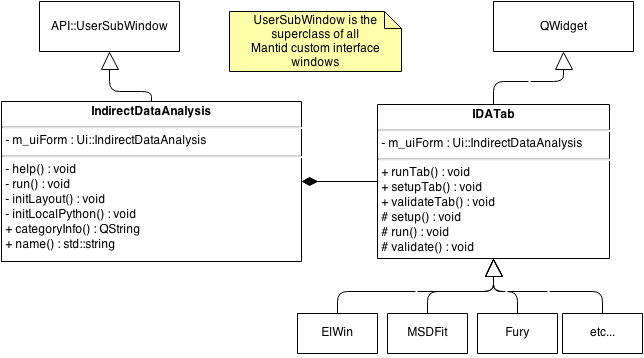
\includegraphics[width=0.7\textwidth]{img/uml/class_diagrams/IDA_structure.png}
\caption{Class diagram for the Indirect Data Analysis GUI.}
\label{fig:IDA-class-diagram}
\end{figure}

As with the convert to energy interface, the layout of the entire GUI is defined in a single XML file which each of the tab objects in the GUI system have a reference too. As of release 3.2 the indirect data analysis interface consists of seven tabs; namely: ElWin, MSDFit, Fury, FuryFit, ConvFit, Calculate Corrections, and Apply Corrections. Each of these have a single class which inherits from a base class called IDATab where the common logic shared between tabs for setting up the tabs, drawing to the mini plot, and loading a nexus file, among other things, is stored.

This approach is much better compared to the one used in the convert to energy interface. The class structure used in the IDA GUI avoids the monolithic class design in convert to energy and separates the implementation logic specific to each routine from the rest of the system while still allowing common code to be shared. However, this structure could still be improved further to remove the reliance on a single GUI file for the defining the interface.

\subsubsection{Indirect Bayes GUI Overview}
\label{subsubsec:Bayes-GUI-Overview}
The GUI structure for the Bayes interface again follows a similar structure to the convert to energy and indirect data analysis interfaces, but takes the abstraction a step further. Like the interfaces discussed before this interface has a single parent class called IndirectBayes which defines the window and a collection of concrete classes paired with each of the tabs which inherit from an abstract base class called IndirectBayesTab which implements the common functionality each tab. 

\begin{figure}[H]
\centering
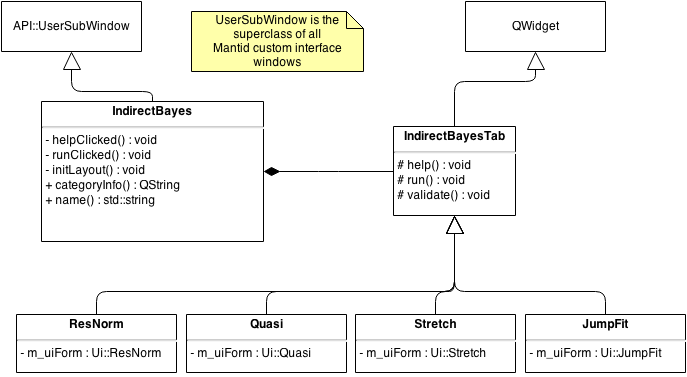
\includegraphics[width=0.7\textwidth]{img/uml/class_diagrams/Bayes_structure.png}
\caption{Class diagram for the Indirect Bayes GUI.}
\label{fig:indirect-bayes-gui}
\end{figure}

The key difference between the two is that instead of the interface being defined in a single UI file, the main window and each of the tabs are defined in separate UI files. This is a subtle difference, but one which provides an enormous benefit to the development process. Splitting the UI into multiple files makes the interface more maintainable as a single tab may be worked on individually without affecting the others. If, for example, a tab needs to be removed or move to a different part of the system it can be easily moved by removing its inclusion in the main window (defined by IndirectBayes).

\subsection{An Example of Basic Data Analysis}
Once a file has been reduced using the convert to energy interface as described in section \ref{sec:energy-transfer} it can be used as input to the various data analysis routines. This section shows a couple of examples of using the Indirect Data Analysis interface with a reduced workspace. Figure \ref{fig:iris-ida-elwin} shows an example of running ElWin to examine the elastic window of an IRIS reduced workspace created from the convert to energy reduction routine. This interface includes a miniplot which shows the first spectrum of the workspace to help pick sensible values for the ranges.

\begin{figure}[H]
\centering
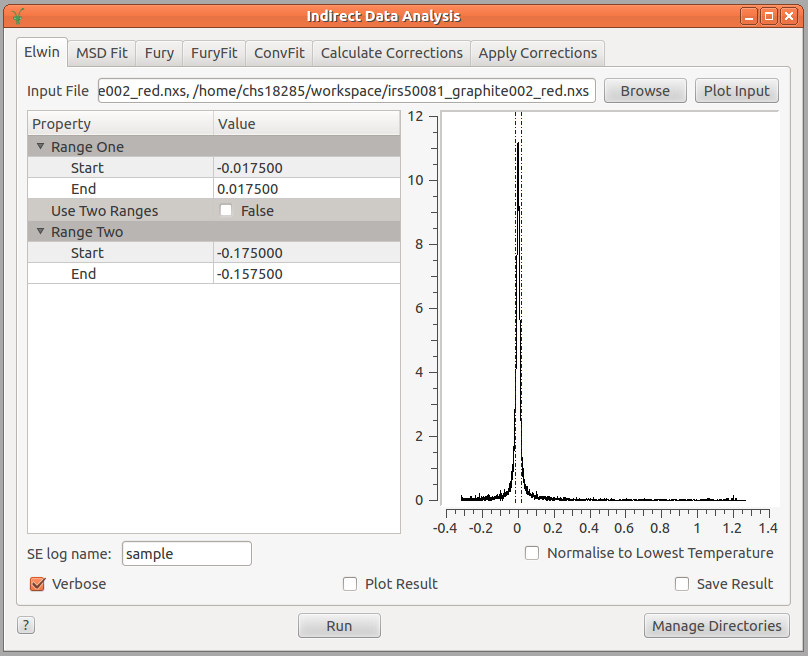
\includegraphics[width=0.6\textwidth]{img/iris-ida-elwin.png}
\caption{Using a reduced workspace with ElWin in release 3.2.}
\label{fig:iris-ida-elwin}
\end{figure}

\begin{figure}[H]
\centering
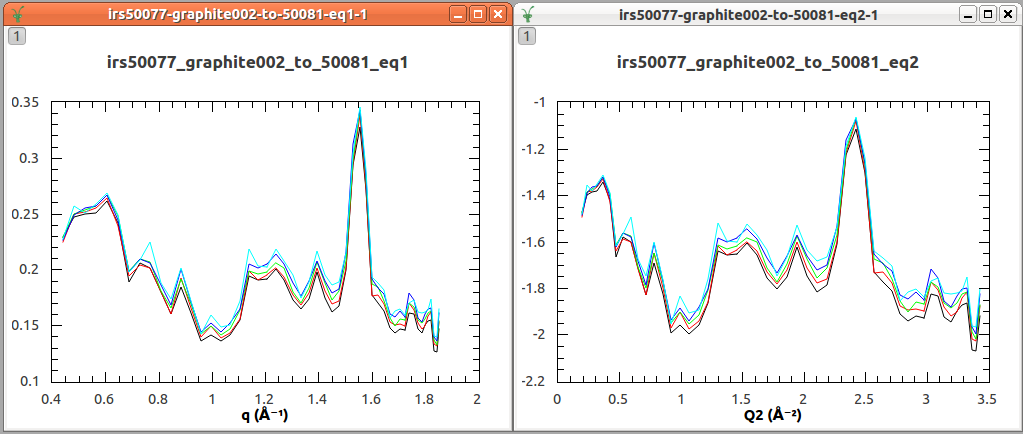
\includegraphics[width=0.9\textwidth]{img/iris-ida-elwin-output.png}
\caption{Plots of the output workspaces from ElWin.}
\label{fig:iris-ida-elwin}
\end{figure}

The \*\_eq2 file created by the routine can be passed to the MSDFit routine to perform a linear fit to the data over all spectra. Again, the miniplot can be used to select the range used with the data. Clicking the run button will fit to just the first spectrum, allowing the user to "get a feel" for the range to be used with the data. Running a sequential fit will use the same range an perform a sequential fit across all spectra in the workspace.

\begin{figure}[H]
\centering
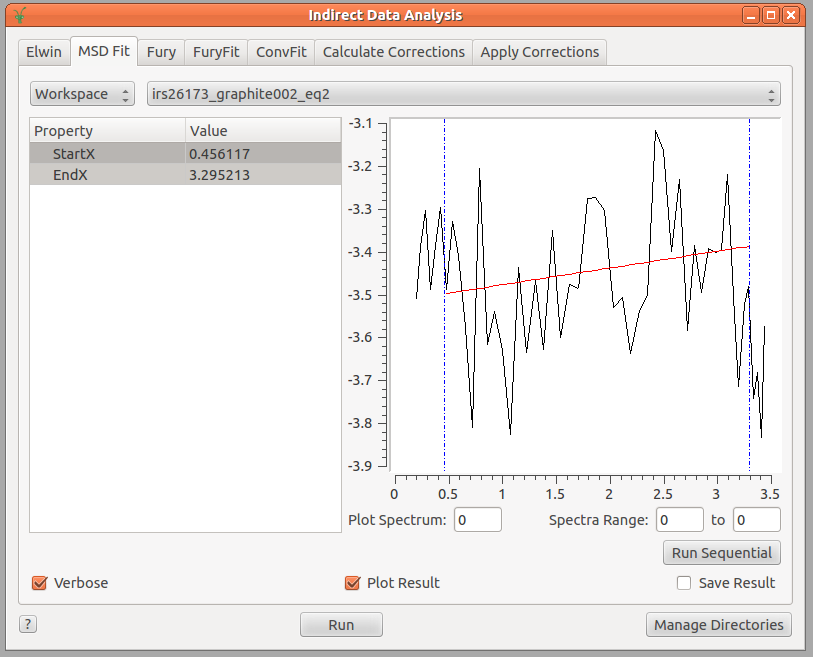
\includegraphics[width=0.6\textwidth]{img/iris-ida-msd.png}
\caption{Using an \*\_eq2 workspace output from ElWin as input to MSDFit.}
\label{fig:iris-ida-msd}
\end{figure}

\begin{figure}[H]
\centering
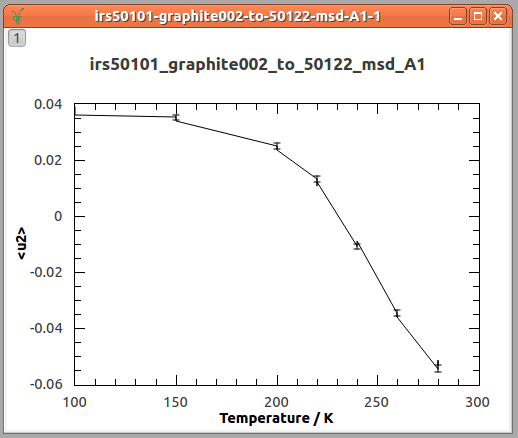
\includegraphics[width=0.5\textwidth]{img/iris-ida-msd-output.png}
\caption{Resulting parameter workspace from MSDFit.}
\label{fig:iris-ida-msd}
\end{figure}

The ConvFit interface (section \ref{subsubsec:convfit}) can be used to separate the instrument resolution from the $S(\mathbf{Q}, \omega)$ function by fitting a convolution of the resolution and the appropriate model to the data. A screen shot of the ConvFit interface is shown in figure \ref{fig:iris-ida-convfit}. This interface has lots of configurable options for the model that is to be convolved with the resolution, but works on similar principle to the MSDFit interface. 

The run button at the bottom of the screen is used to perform a single fit to the data which also updates the parameters for the model in the properties browser. This is useful because it allows the user to choose parameters close to the appropriate value, then tighten them up before fitting all spectra. Once the user is happy with the fit parameters for a single spectrum (shown in the mini plot) the sequential fit button can be used to fit all of the spectra.

\begin{figure}[H]
\centering
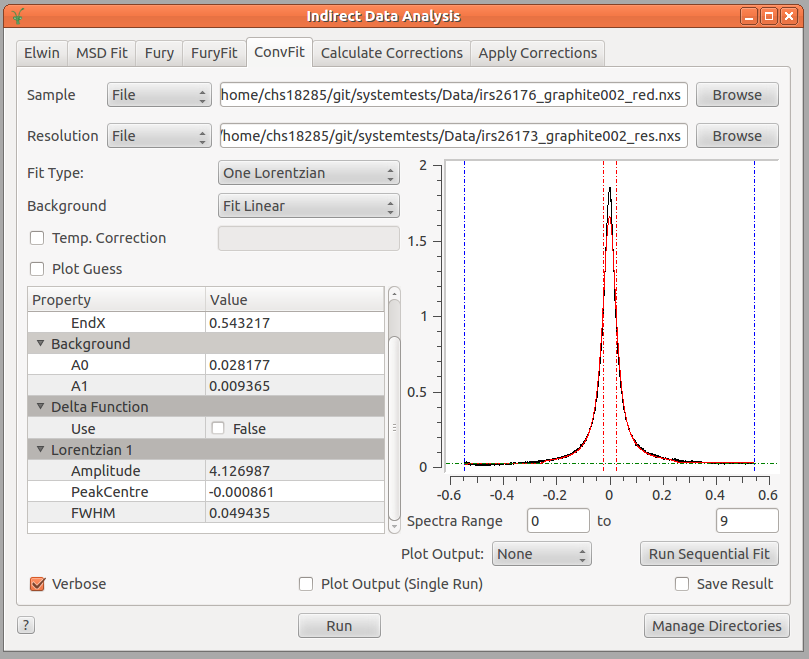
\includegraphics[width=0.5\textwidth]{img/iris-ida-convfit.png}
\caption{Screen shot of using the ConvFit interface to fit a single Lorentzian to the data.}
\label{fig:iris-ida-convfit}
\end{figure}

\subsection{An Example of Advanced Data Analysis}
The Bayesian fitting routines also operate on the reduced data create from Indirect Convert to Energy. Using an example reduced workspace from the IRIS instrument we can run the ResNorm program to generate a normalisation group workspace as shown in screen shot \ref{fig:iris-bayes-resnorm}. As with other interfaces, the mini plot shows the first spectrum in the workspace and can be used to select the range used for binning. The resolution workspace is one that has been generated from the Calibration tab on the Convert to Energy interface (see section \ref{subsec:c2e-calibration}).

\begin{figure}[H]
\centering
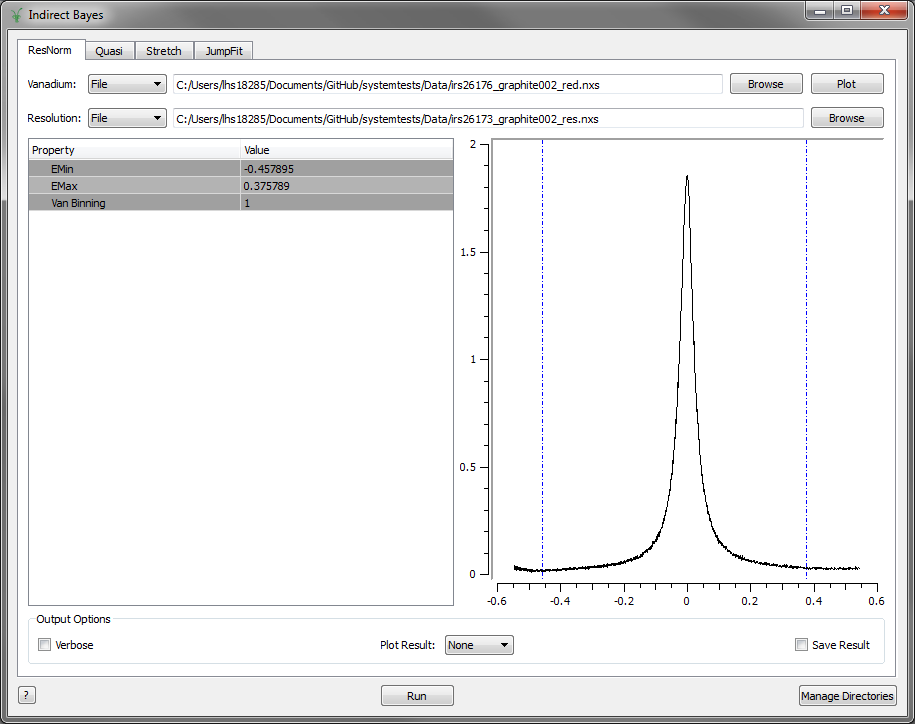
\includegraphics[width=0.5\textwidth]{img/iris-bayes-resnorm.png}
\caption{Screen shot of using the ResNorm interface in release 3.2.}
\label{fig:iris-bayes-resnorm}
\end{figure}

The Quasi routine offers a complementary alternative to the ConvFit routine. The workspace output from ResNorm can be used as input to the Quasi routine. Like the ConvFit routine this takes both a reduced sample and resolution file. The model to be fitted can be configured using the various options for the background and type of peak before running. Figure \ref{fig:iris-bayes-quasi} shows an example of using the interface in release 3.2.

\begin{figure}[H]
\centering
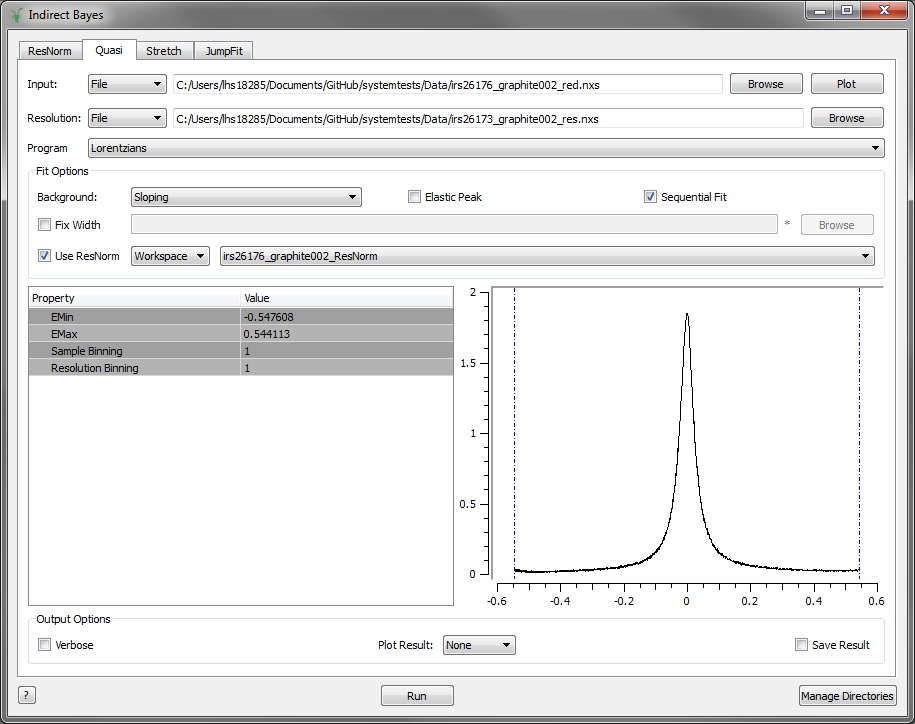
\includegraphics[width=0.5\textwidth]{img/iris-bayes-quasi.png}
\caption{Fitting a model to some reduced data from IRIS using the Quasi interface.}
\label{fig:iris-bayes-quasi}
\end{figure}

As a final example, shown in figure \ref{fig:iris-bayes-jumpfit}, the workspace of fit parameters output from Quasi can be used as direct input to the JumpFit routine. This automatically finds the width parameters within the workspace and allows the user to select which one to fit. The user can choose between any of the models defined for diffusion. Future releases hope to add support using a custom function string as the model for fitting.

\begin{figure}[H]
\centering
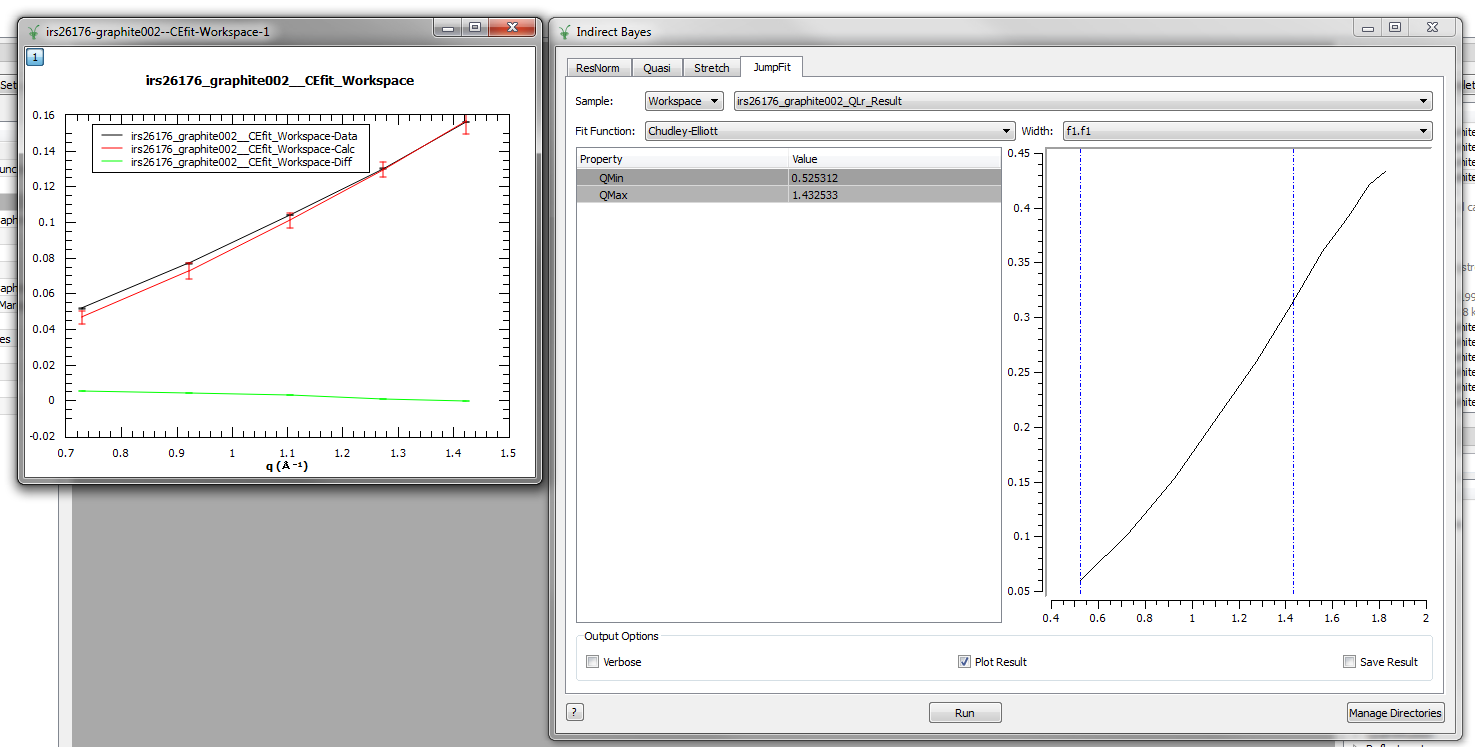
\includegraphics[width=0.7\textwidth]{img/iris-bayes-jumpfit.png}
\caption{Using JumpFit on the output from the Quasi interface.}
\label{fig:iris-bayes-jumpfit}
\end{figure}


\section{Materials Modelling}
\label{sec:simulation}
Another important part of experimental analysis involved the comparison of experimental results against theoretical predictions. This is an area of development that is only just beginning and there is only a very small amount of support implemented so far.

\subsection{Indirect Simulation}
Indirect Simulation is a new interface for release 3.2 that splits the basic nMolDyn loader that is currently in Mantid off from it's original location in the Indirect Load ASCII interface. This interface is planned to be a place to expose simulation routines to the GUI level, such as adding interface support for the Sassena routines already in Mantid in future releases.

\subsection{nMolDyn}
The nMolDyn interface that currently exists is a very simple routine to load data from a nMolDyn simulation files into a Mantid workspace. In future releases of Mantid it is proposed to attempt to properly integrate support for the nMolDyn python libraries into Mantid, providing a much richer selection of tools for the user. The code for this can be found the IndirectMolDyn.py file in the Inelastic scripts folder.

\subsection{Density Of States}
The DensityofStates algorithm was a new addition to the 3.1 release of Mantid and does not currently have GUI support. It provides loading algorithm for .castep and .phonon files generated by CASTEP simulation program and create workspaces with both total and partial density of states data. Further support for CASTEP is planned in future releases. The code for this file can be found in DensityOfStates.py file under python algorithm plugins section in the Mantid install.

\section{Planning For the Future}
This section outlines outstanding work required to fully support indirect geometry instruments within Mantid. This section is not meant as a ``set in stone'' plan for further development but is meant as guide for future development work in the area and a loose record of user and project requirements all of which are subject to change.

\subsection{Conversion of Existing Routines to Algorithms and Work-Flow Algorithms}
Now that a large proportion of the code base required for data reduction and analysis of indirect geometry spectroscopy has been incorporated into Mantid, it is time to move forward with consolidating the existing code base we already have. As already mentioned in the earlier sections of this document most of the code base is either using the old style reducer-reduction step framework or is in the form of simple python scripts which are both not sufficiently documented and (largely) untested.

Ideally, the Indirect framework should take advantage of the core concept of the Mantid framework: algorithms. An algorithm in Mantid is defined as being a set of code that performs some operation on a workspace. Algorithms are well documented (both for the user and the development team) and are the preferred common interface for performing actions in Mantid.

There are two types of algorithms in Mantid. Normal algorithms are simply ones which perform some operation on a workspace, such as ConvertUnits or Fit or Load. The second type is called a work flow algorithm. This is an algorithm that performs no direct manipulation of a workspace itself, but executes a collection of algorithms other algorithms in order to perform some larger task. An example of such an algorithm would be DgsReduction or ReflectometryReductionAutoOne. The benefits of the latter are that: 

\begin{itemize}
\item Large operations get broken do into smaller, more easily understood operations which already have algorithms defined which are used by multiple research groups and facilities and have become tried and tested.

\item Algorithms and work flow algorithms still support inheritance like the reducer objects

\item They are easily unit testable, meaning that automated checking of the integrity of each part of the reduction is handled automatically by the build servers, which helps prevent errors.

\item They are by default exposed through the Mantid simple python API like any other algorithm which means they can easily be chained together with other algorithms and can be run even if the interface is broken.

\item As of release 3.2 the ability to track the history of a work flow algorithm and it's child algorithms has been added, allowing scientists to see exactly what operations have been performed on a workspace since it entered Mantid.
\end{itemize}

Energy transfer reduction and diffraction reduction are both prime candidates for work flow algorithms. Neither of these routines actually perform any real direct manipulation of the workspaces they reduce themselves, but delegate all of the operations to existing Mantid algorithms within the reduction steps. Converting this would be a delicate and large job, but not necessarily difficult. The basic outline of both reductions is already documented in diagrams \ref{fig:c2e-energy-transfer-activity-diagram} and \ref{fig:diffraction-class-diagram} respectively. This, along with the actual code (which is reasonably we documented and formatted) should be enough for an easy transition to a work flow algorithm for each type of reduction.

Some of the large reduction steps would also benefit from being converted to work flow algorithms in there own right, particularly the reduction steps which are larger and shared between both reducer classes. Prime examples would be the LoadData and HandleMonitor steps which are both complex enough that they could be converted to work flow algorithms.

To convert the existing reduction routines into work flow algorithms, I would suggest first writing detailed unit tests to cover all of the reduction steps. The full energy conversion reduction itself is already covered by automated system testing to periodically check the integrity of the results. The next step would be to concrete reducer classes to be algorithms one at a time and hooking them up with the relevant GUI. The final step would be to convert the reduction steps to either be algorithms or work flow algorithms in there own right or to simply incorporate the code into the reduction work flows themselves. Work flow algorithms essentially just a class and therefore support inheritance which means common code between both reducers should end up being stored in a common base class.

Outside of the main reducers, the main other scripts used throughout the Indirect framework should be converted to be proper Mantid algorithms for the reasons listed above. However, many of these routines are considerably simpler than the reducer work flows and for many of them it may be best just to convert them to plain algorithms. Many routines, such as the the data analysis fitting routines MSDFit, FuryFit and ConvFit share very similar functionality with only a few slight differences between implementations. In the case of the routines listed, they all essentially pass a function string to PlotPeakByLogValue or Fit and convert the output table workspace to a matrix workspace of parameters. These could probably be reimplemented as a single algorithm which handles the fitting for all three routines. Consolidating the code base in this way could also be done with the Bayesian fitting routines Quasi and Stretch but should only be done after converting the Fortran modules (see section \ref{subsec:convert-fortran}).

\subsection{Better Automated Test Coverage}
One key development area in which the indirect framework is lacking is a good level of test coverage. At the time of writing the Mantid development system carries out two types of automated testing: unit tests and system tests. Unit tests are designed to be quick to execute and run frequently. System tests are typically longer and check the the integrity of the system as a whole.

Currently the only automated testing that is carried out by the system is a through the system tests. These tests run one or more of the routines and compares the results against a reference file to check that the results still match after changes have been made to the framework. This is essential to checking that nothing gets broken in the core parts of the system, such as the energy transfer and diffraction reduction but in no way covers every aspect of the system. There are currently no unit tests covering the any of the scripts mentioned in the previous sections, except for algorithms such as SofQW, SofQWMoments, and DensityOfStates.

A small maintenance project needs to be undertaken to increase the automated test coverage across all areas of the indirect framework. Ideally, every function, routine, reducer, and reduction step should have a unit test or suite of tests covering it. Improving the test coverage offers little direct benefit to the users of the system, but will make it easier to identify and prevent errors within the system ultimately leading to more time spent on productive development and less time fixing bugs.

Additionally, more system tests need to be added to more extensively cover some of the more common use cases between different routines. For example, there is currently a test for running Fury and passing it to FuryFit, but no such test for running Quasi and passing the result to JumpFit.

\subsection{Improved GUI structure and design}
\label{subsec:GUI-Improvements}
All of the interfaces for indirect data reduction and analysis share common themes in GUI design (except Diffraction, largely due to its simplicity). All of them share the same basic format: one tab for each routine, input files at the top of the window, parameters in the middle and a mini plot if required, output options at the bottom followed by the run button.

Having a consistent feel across all interfaces is extremely important in making it easy for users to learn to use the software and there is plenty that could be done to improve this within the existing GUIs. However, a more pertinent issue, and one that should be tackled first, is the repetition of common code both between interfaces and between individual tabs. Notice that the class diagrams in the GUI overviews in sections \ref{subsec:c2e-gui-overview}, \ref{subsubsec:Bayes-GUI-Overview}, and \ref{subsubsec:IDA-GUI-Overview} share a very similar class structure.

Future development should aim to unify this repeatable structure into a using a single common class hierarchy with abstract base classes sharing functionality that is shared between all of the interfaces. This would include, for example:

\begin{itemize}
\item Mini plot set-up, drawing, updating, and management routines.
\item Common file loading and pre-processing calls.
\item Algorithm instantiation, execution, and error handling code.
\end{itemize}

\begin{figure}[H]
\centering
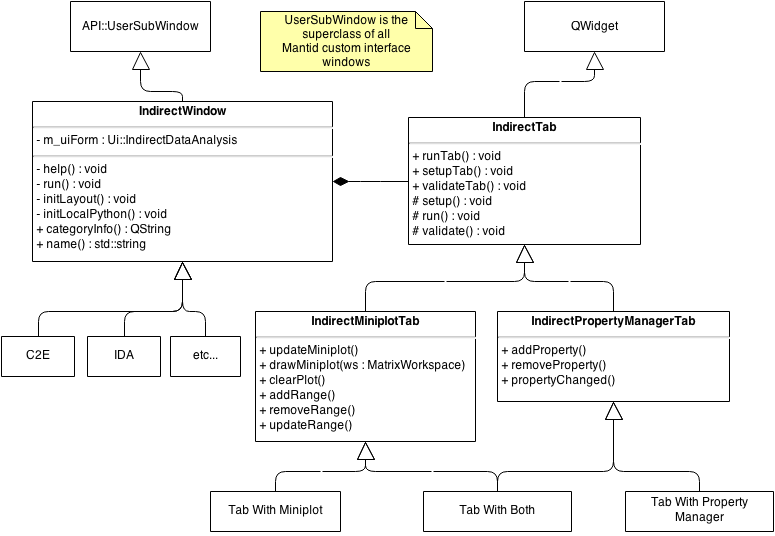
\includegraphics[width=0.7\textwidth]{img/uml/class_diagrams/IndirectGUI_structure_proposed.png}
\caption{Class diagram for what a refactored GUI hierarchy might look like.}
\label{fig:indirect-gui-proposed}
\end{figure}

A refactored GUI class hierarchy could look something like diagram \ref{fig:indirect-gui-proposed}. This shows that all of the interface classes share a common abstract base class. More specific abstract base classes then implement functionality which is dependant upon what is contained within the interface (e.g. a mini plot) until reaching the concrete class which contains the exact details of setting up, validating and running a specific routine. This allows us to share common code that has already been written multiple times throughout the various interfaces, but have it defined in only one place. 

The GUI window itself is a abstract base single class with a single interface file. All of the indirect GUIs follow the same pattern: tabs for each routine with a run, help, and manage directories buttons at the bottom of the window. The name and specific settings of the window can be then be implemented using a concrete derived class for each individual interface.

Furthermore, to expand on the last bullet point above, the interface currently executes python routines by creating a string of python code with the calls to each routine and all of the parameters it requires. This approach is both fiddly and error prone. It is easy to build a string which is not formatted correctly in some subtle way which leads to broken options and code paths.

A much better approach would be to convert the existing routines to Mantid algorithms (as discussed in the previous section) and to then use Mantid's algorithm runner class to execute the desired algorithm on the separate thread. This approach makes it much harder to break because any errors in preparing the algorithm are likely to be raised at compile time as opposed to run time (as with python scripts). It also means that the errors occurring during runtime can be caught by the interface (which cannot be done using the current method) and handled appropriately. 

The code to handle setting up and executing algorithms would not be overly complicated, Mantid already has an algorithm runner class, but it could be adapted further if required, and could be written into the base class of the GUI hierarchy. This would allow it to be written once and used everywhere. 

One final thing to note is that this should wait until the energy conversion for direct geometry instruments is split from the indirect geometry interface so that restructuring the interface does not effect development in that area.

\subsection{Simulation Support in Mantid}
Support for simulation is an area in which there has been little development so far for indirect, but would be a useful addition to our existing collection. As mentioned in section \ref{sec:simulation} there is a small amount of existing support for some simulation programs within Mantid. There are currently loaders for the output of CASTEP, Sassena, and nMOLDYN simulations. In the most recent release, a new interface was created as a place to integrate simulation programs into Mantid's GUI.

One current goal in the development of Mantid is to attempt to integrate the open source nMOLDYN library into Mantid and package it with the distribution of the project. This would not only further enrich the existing Python API available in Mantid, but would also provided us with an extensive, reliable molecular dynamics simulation package with which to build on.

Approval has already been given to include the library as the functionality it provides has been deemed generic enough to be beneficial to a significant number of Mantid users. The first step in this project would be to separate the the nMOLDYN library from its dependencies and examine what libraries it requires that Mantid does not already have support for. Assuming that there are then no dependencies that cannot be shipped directly with Mantid, further development could then focus on building useful simulation routines for comparison with experimental data in conjunction with the requirements of instrument scientists.

\subsection{Conversion of Remaining Fortran Routines}
\label{subsec:convert-fortran}
As mentioned in several sections through out the documentation of existing development, are several routines that still rely on Fortran routines that have been directly assimilated into Mantid using the F2Py package. This has allowed quick integration of routines needed for analysis, but it is not a cross platform solution, is not well documented, and the current code is incredibly difficult to decipher.

A long term goal would be to convert these existing, tried and tested routines into well documented, thoroughly unit tested C++ or python code which utilises the some of the existing fitting routines that are already present inside Mantid. As mentioned in the previous section, some of the functionality is repeated inside the code for Quasi and Stretch and it may be the case that common code could be merged during the conversion.

The biggest difficulty with this is that it will require a sizeable chunk of a developers time and a good understanding of Fortran and what the underlying code is doing in order to convert the routines and write thorough tests for the converted code to ensure the fitting is good enough to match the existing Fortran while still matching the process described in the references.

There are currently four routines that are still in Fortran code: the three Bayes programs (ResNorm, Quasi, and Stretch) and the cylindrical absorption corrections program used in the calculate corrections routine. There are additional Fortran based routines in the for multiple scattering (see section \ref{subsec:multiple-scattering}) which will also need to be ported to Mantid in future releases.

\subsection{Support for VESUVIO}
Due to the uniqueness of the instrument, VESUVIO is currently not officially supported by the Mantid framework. Significant development work has already been undertaken add the data reduction and analysis routines that VESUVIO requires into the Mantid framework. The majority of the modifications to the framework have already been implemented, but some areas such as multiple scattering corrections \cite{mayers2002multiple} and global fitting are still incomplete. Besides this there is currently no GUI support for VESUVIO within Mantid. Once all parties involved are in happy with the state of the prototype reduction and analysis routines in Mantid work can begin on the developing a GUI. Broadly, this would require a separate interface under the indirect section of Mantid, loosely separated in to the following sections:

\begin{itemize}
\item \textbf{Loading:} This would provide a user interface for using the LoadVesuvio algorithm to get raw data into Mantid as well as providing plotting functions for examining the captured time-of-flight data.

\item \textbf{Corrections:} The corrections interface would provide a user interface for calculating both multiple scattering \cite{mayers2002multiple} and gamma background \cite{mayers2011calculation} corrections and applying them to data loaded in the first tab.

\item \textbf{Fitting:} The fitting interface is the most complex in the series. This will provide support for setting up a fit using the same procedures used in the Ref. \cite{mayers2010user}, but in a more user friendly manner than the current implementation achieves. This would provide support for both the Gaussian and Gram-Charlier functions with the ability to easily set the intensity constraints and hermite coefficients.
\end{itemize}

Additional sections may also be required, such as interfaces for the global fitting and fitting data directly in y-space, but a full design will wait until after the framework behind VESUVIO analysis is finalised.

\subsection{Additional Support for TOSCA}
TOSCA has had several previous incarnations before its current set up, and has been known as TFXA in the past \cite{penfold1986isis, parker1997tosca, bowden2000tosca, colognesi2002tosca}. Mantid currently only has the most recent set up for the instrument defined. The older incarnations should be able to be supported fairly easily using tools already in the Mantid framework. The geometry of each instrument is defined using a instrument definition file XML file. This XML file has a date valid from and to attribute that allows Mantid to figure out at the load time what instrument definition to use with a particular run. Each older incarnation can be defined using this attribute by setting it to be valid within the appropriate date range, meaning the correct definition for TOSCA will be loaded at runtime for each sample reduced based on the age of the sample run. 

A prototype instrument definition file has already been tested for TFXA, but additional work will be required to properly support the full range of TOSCA's history. In particular a full description of the geometry of the instrument in 3D space is required for each prior incarnation for an accurate definition.

Another requirement by the TOSCA team is to add support for the Renishaw Ramen spectroscopy instrument which is used to perform Ramen spectroscopy and neutron spectroscopy simultaneously. The data from the Renishaw instrument can currently be imported into Mantid through the ASCII loading algorithms already in place, but this is an awkward process. A better approach would be to provide a way to store the runs on the TOSCA data archive and then provide procedures for loading the run directly from the archive as is currently done for regular neutron sample runs on TOSCA.

\subsection{Improved Support for Other Facilities}
Officially the framework we currently have supports both the SNS and ISIS. However, there has been a lot of development during the last release to further support for the ILL within Mantid. One of the goals of future development should be to integrate the existing loading and reduction routines with the existing GUI. This would eventually lead to the removal of the Indirect Load ASCII interface which would no longer be required.

\subsection{Multiple Scattering Support}
\label{subsec:multiple-scattering}
The multiple scattering routines from the MODES package are the last major parts that have not been ported from the MODES application in one form or another. There are two different multiple scattering routines called MuscatData and MuscatFunc which were originally part of the MODES package as the program MINUS which in turn was adapted from the DISCUS program \citep{wshowells2010, mjohnson1974}. Both routines work with both flat and cylindrical geometries. The difference between the two is MuscatData uses takes $S(Q,w)$ workspace as input, while MuscatFunc just uses a set of specified parameters from the user. 

Ideally these routines should be converted from Fortran to C++ code first before including them in Mantid, but if demand is high they can be included in the GUI in the same way Bayes and cylindrical corrections works using the F2Py package. There has already been some existing work to import them into Mantid, but the current versions do not work. Recently, there has also been a goal outlined by the scientific steering committee to provide a general framework for multiple scattering corrections within Mantid. At the time of writing it is uncertain whether the planned implementation of this will be compatible with the existing methods used by the MODES routines.

\section*{Acknowledgements}
The author would like to thank S. Mukhopadhyay for her assistance in the writing of this report and in particular for her guidance and support with the theory section of the document. Additional thanks W.S. Howells for his enumerable contributions to the development of the indirect geometry section, particularly in regards to QENS analysis, and F. Fernandez-Alonso for his constructive comments and criticisms.
\bibliographystyle{unsrtnat_corrected}
\bibliography{refs}
\end{document}
